% memorder/memorder.tex

\QuickQuizChapter{chp:memorder:Memory Ordering}{Memory Ordering}
\OriginallyPublished{Chapter}{chp:memorder:Memory Ordering}{Linux Kernel Memory Barriers}{kernel.org}{Howells2009membartxt}
\OriginallyPublished{Chapter}{chp:memorder:Memory Ordering}{A formal kernel memory-ordering model}{Linux Weekly News}{JadeAlglave2017LWN-LKMM-1,JadeAlglave2017LWN-LKMM-2}
%
\Epigraph{The art of progress is to preserve order amid change and to preserve change amid order.}{\emph{Alfred North Whitehead}}

Causality and sequencing are deeply intuitive, and hackers often
tend to have a much stronger grasp of these concepts than does
the general population.
These intuitions can be extremely powerful tools when writing, analyzing,
and debugging both sequential code and parallel code that makes
use of standard mutual-exclusion mechanisms, such as locking and
RCU.
Unfortunately, these intuitions break down completely in face of
code that fails to use standard mechanisms, one important example
of course being the code that implements these standard mechanisms.
This chapter will help you gain an understanding of memory ordering
sufficient to implement synchronization primitives and other
performance-critical code.

@@@ roadmap @@@

\section{Ordering: Why and How?}
\label{sec:memorder:Ordering: Why and How?}

One motivation for memory ordering can be seen in the trivial-seeming
litmus test in
Listing~\ref{lst:memorder:Memory Misordering: Store-Buffering Litmus Test}
(\path{C-SB+o-o+o-o.litmus}),
which at first glance might
appear to guarantee that the \co{exists} clause never triggers.\footnote{
	Purists would instead say that the \co{exists} clause is
	never \emph{satisfied}, but we use ``trigger'' here by
	analogy with assertions.}
After all, if \nbco{0:r2=0} as shown in the \co{exists} clause,\footnote{
	That is, Thread~\co{P0()}'s instance of local variable \co{r2}
	equals zero.
	See Section~\ref{sec:formal:Anatomy of a Litmus Test}
	for documentation of litmus-test nomenclature.}
we might hope that Thread~\co{P0()}'s
load from~\co{x1} must have happened before Thread~\co{P1()}'s store to~\co{x1},
which might raise
further hopes that Thread~\co{P1()}'s load from~\co{x0} must happen after
Thread~\co{P0()}'s store to~\co{x0}, so that \nbco{1:r2=2},
thus not triggering the \co{exists} clause.
The example is symmetric, so similar reasoning might lead
us to hope that \nbco{1:r2=0} guarantees that \nbco{0:r2=2}.
Unfortunately, the lack of memory barriers dashes these hopes.
The CPU is within its rights to reorder
the statements within both Thread~\co{P0()} and Thread~\co{P1()},
even on relatively strongly ordered systems such as x86.

\begin{listing}[tbp]
{ \scriptsize
\begin{verbbox}[\LstLineNo]
C C-SB+o-o+o-o
{
}

P0(int *x0, int *x1)
{
  int r2;

  WRITE_ONCE(*x0, 2);
  r2 = READ_ONCE(*x1);
}


P1(int *x0, int *x1)
{
  int r2;

  WRITE_ONCE(*x1, 2);
  r2 = READ_ONCE(*x0);
}

exists (1:r2=0 /\ 0:r2=0)
\end{verbbox}
}
\centering
\theverbbox
\caption{Memory Misordering: Store-Buffering Litmus Test}
\label{lst:memorder:Memory Misordering: Store-Buffering Litmus Test}
\end{listing}

\QuickQuiz{}
	The compiler can also reorder Thread~\co{P0()}'s and
	Thread~\co{P1()}'s memory accesses in
	Listing~\ref{lst:memorder:Memory Misordering: Store-Buffering Litmus Test},
	right?
\QuickQuizAnswer{
	In general, compiler optimizations carry out more extensive
	and profound reorderings than CPUs can.
	However, in this case, the volatile accesses in
	\co{READ_ONCE()} and \co{WRITE_ONCE()}
	prevent the compiler from reordering.
	And also from doing much else as well, so the examples in this
	section will be making heavy use of
	\co{READ_ONCE()} and \co{WRITE_ONCE()}.
	% @@@ forward reference to a section describing READ_ONCE()
	% @@@ and WRITE_ONCE().
} \QuickQuizEnd

This willingness to reorder can be confirmed using tools such as
\co{litmus7}~\cite{Alglave:2014:HCM:2594291.2594347},
which found that the counter-intuitive ordering happened
314 times out of 100,000,000 trials on my x86 laptop.
Oddly enough, the perfectly legal outcome where both loads return the
value 2 occurred less frequently, in this case, only 167 times.\footnote{
	Please note that results are sensitive to the exact hardware
	configuration,
	how heavily the system is loaded, and much else besides.}
The lesson here is clear: Increased counterintuitivity does not necessarily
imply decreased probability!
% Run on June 23, 2017:
% litmus7 -r 1000 -carch X86 C-SB+o-o+o-o.litmus
% Test C-SB+o-o+o-o Allowed
% Histogram (4 states)
% 314   *>0:r2=0; 1:r2=0;
% 49999625:>0:r2=2; 1:r2=0;
% 49999894:>0:r2=0; 1:r2=2;
% 167   :>0:r2=2; 1:r2=2;

The following sections show exactly where this intuition breaks down,
and then puts forward a mental model of memory barriers that can help
you avoid these pitfalls.

Section~\ref{sec:memorder:Why Hardware Misordering?}
gives a brief overview of why hardware misorders memory accesses, and then
Section~\ref{sec:memorder:How to Force Ordering?}
gives an equally brief overview of how you can thwart evil hardware
misordering schemes.
Finally, Section~\ref{sec:memorder:Basic Rules of Thumb}
lists some basic rules of thum, which will be further refined in
later sections.

\subsection{Why Hardware Misordering?}
\label{sec:memorder:Why Hardware Misordering?}

But why are memory barriers needed in the first place?
Can't CPUs keep track of ordering on their own?
Isn't that why we have computers in the first place, to keep track of things?

Many people do indeed expect their computers to keep track of things,
but many also insist that they keep track of things quickly.
However, as seen in Chapter~\ref{chp:Hardware and its Habits},
one difficulty that modern computer-system vendors face is that
the main memory cannot keep up with the CPU---modern CPUs can execute
hundreds of instructions in the time required to fetch a single variable
from memory.
CPUs therefore sport increasingly large caches, as seen back in
Figure~\ref{fig:cpu:System Hardware Architecture}, which means that
although the first load by a given CPU from a given variable will
result in an expensive \emph{cache miss} as was discussed in
Section~\ref{sec:cpu:Cache Misses}, subsequent
repeated loads from that variable by that CPU might execute
very quickly because the initial cache miss will have loaded that
variable into that CPU's cache.

However, it is also necessary to accommodate frequent concurrent stores
from multiple CPUs to a set of shared variables.
In cache-coherent systems, if the caches hold multiple copies of a given
variable, all the copies of that variable must have the same value.
This works extremely well for concurrent loads, but not so well for
concurrent stores:  Each store must do something about all
copies of the old value (another cache miss!), which, given the finite
speed of light and the atomic nature of matter, will be slower
than impatient software hackers would like.

\begin{figure}[tb]
\centering
\resizebox{2.5in}{!}{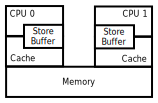
\includegraphics{memorder/SystemArchSB}}
\caption{System Architecture With Store Buffers}
\label{fig:memorder:System Architecture With Store Buffers}
\end{figure}

CPUs therefore come equipped with store buffers, as shown in
Figure~\ref{fig:memorder:System Architecture With Store Buffers}.
When a given CPU does a store to a variable that
is not present in that CPU's cache, then the new value
is instead placed in that CPU's store buffer.
The CPU can then proceed immediately, without having to wait for the
store to do something about all the old values of that variable
residing in other CPUs' caches.

\begin{figure}[htb]
\centering
\resizebox{3in}{!}{
\includegraphics{cartoons/r-2014-Out-of-order}}
\caption{CPUs Can Do Things Out of Order}
\ContributedBy{Figure}{fig:memorder:CPUs Can Do Things Out of Order}{Melissa Broussard}
\end{figure}

Although store buffers can greatly increase performance,
they can cause instructions and memory references to execute out
of order, which can in turn cause serious confusion, as illustrated in
Figure~\ref{fig:memorder:CPUs Can Do Things Out of Order}.
In particular, these store buffers can cause the memory misordering
shown in the store-buffering litmus test in
Listing~\ref{lst:memorder:Memory Misordering: Store-Buffering Litmus Test}.

\begin{table*}
\small
\centering\OneColumnHSpace{-0.1in}
\begin{tabular}{r||l|l|l||l|l|l}
	& \multicolumn{3}{c||}{CPU 0} & \multicolumn{3}{c}{CPU 1} \\
	\cline{2-7}
	& Instruction & Store Buffer & Cache &
		Instruction & Store Buffer & Cache \\
	\hline
	\hline
	1 & (Initial state) & & \tco{x1==0} &
		(Initial state) & & \tco{x0==0} \\
	\hline
	2 & \tco{x0 = 2;} & \tco{x0==2} & \tco{x1==0} &
		\tco{x1 = 2;} & \tco{x1==2} & \tco{x0==0} \\
	\hline
	3 & \tco{r2 = x1;} (0) & \tco{x0==2} & \tco{x1==0} &
		\tco{r2 = x0;} (0) & \tco{x1==2} & \tco{x0==0} \\
	\hline
	4 & (Read-invalidate) & \tco{x0==2} & \tco{x0==0} &
		(Read-invalidate) & \tco{x1==2} & \tco{x1==0} \\
	\hline
	5 & (Finish store) & & \tco{x0==2} &
		(Finish store) & & \tco{x1==2} \\
\end{tabular}
\caption{Memory Misordering: Store-Buffering Sequence of Events}
\label{tab:memorder:Memory Misordering: Store-Buffering Sequence of Events}
\end{table*}

Table~\ref{tab:memorder:Memory Misordering: Store-Buffering Sequence of Events}
shows how this memory misordering can happen.
Row~1 shows the initial state, where CPU~0 has \co{x1} in its cache
and CPU~1 has \co{x0} in its cache, both variables having a value of zero.
Row~2 shows the state change due to each CPU's store (lines~9 and~18 of
Listing~\ref{lst:memorder:Memory Misordering: Store-Buffering Litmus Test}).
Because neither CPU has the stored-to variable in its cache, both CPUs
record their stores in their respective store buffers.

\QuickQuiz{}
	But wait!!!
	On row~2 of
	Table~\ref{tab:memorder:Memory Misordering: Store-Buffering Sequence of Events}
	both \co{x0} and \co{x1} each have two values at the same time,
	namely zero and two.
	How can that possibly work???
\QuickQuizAnswer{
	There is an underlying cache-coherence protocol that straightens
	things out, which will be discussed later.
	% @@@ Add forward reference.
	But if you think that a given variable having two values at
	the same time is surprising, just wait until you get to
	Section~\ref{sec:memorder:Variables With Multiple Values}!
} \QuickQuizEnd

Row~3 shows the two loads (lines~10 and~19 of
Listing~\ref{lst:memorder:Memory Misordering: Store-Buffering Litmus Test}).
Because the variable being loaded by each CPU is in that CPU's cache,
each load immediately returns the cached value, which in both cases
is zero.

But the CPUs are not done yet: Sooner or later, they must empty their
store buffers.
Because caches move data around in relatively large blocks called
\emph{cachelines}, and because each cacheline can hold several
variables, each CPU must get the cacheline into its own cache so
that it can update the portion of that cacheline corresponding
to the variable in its store buffer, but without disturbing any
other part of the cacheline.
Each CPU must also ensure that the cacheline is not present in any other
CPU's cache, for which a read-invalidate operation is used.
As shown on row~4, after both read-invalidate operations complete,
the two CPUs have traded cachelines, so that CPU~0's cache now contains
\co{x0} and CPU~1's cache now contains \co{x1}.
Once these two variables are in their new homes, each CPU can flush
its store buffer into the corresponding cache line, leaving each
variable with its final value as shown on row~5.

\QuickQuiz{}
	But don't the values also need to be flushed from the cache
	to main memory?
\QuickQuizAnswer{
	Perhaps surprisingly, not necessarily!
	On some systems,
	if the two variables are being used heavily, they might
	be bounced back and forth between the CPUs' caches and never
	land in main memory.
} \QuickQuizEnd

In summary, store buffers are needed to allow CPUs to handle
store instructions efficiently, but they can result in
counter-intuitive memory misordering.

But what do you do if your algorithm really needs its memory
references to be ordered?
For example, suppose that you are communicating with a driver using
a pair of flags, one that says whether or not the driver is running
and the other that says whether there is a request pending for that
driver.
The requester needs to set the request-pending flag, then check
the driver-running flag, and if false, wake it up.
Once the driver has serviced all the pending requests that it knows about,
it needs to clear its driver-running flag, then check the request-pending
flag to see if it needs to restart.
This very reasonable approach cannot work unless there is some way
to make sure that the hardware processes the stores and loads in order.
This is the subject of the next section.

\subsection{How to Force Ordering?}
\label{sec:memorder:How to Force Ordering?}

It turns out that there are compiler directives and standard
synchronization primitives (such as locking and RCU)
that are responsible for maintaining the illusion of ordering through use of
\emph{memory barriers} (for example, \co{smp_mb()} in the Linux kernel).
These memory barriers can be explicit instructions, as they are on
ARM, POWER, Itanium, and Alpha, or they can be implied by other instructions,
as they often are on x86.
Since these standard synchronization primitives preserve the illusion of
ordering, your path of least resistance is to simply use these primitives,
thus allowing you to stop reading this section.

\begin{listing}[tbp]
{ \scriptsize
\begin{verbbox}[\LstLineNo]
C C-SB+o-mb-o+o-mb-o
{
}

P0(int *x0, int *x1)
{
  int r2;

  WRITE_ONCE(*x0, 2);
  smp_mb();
  r2 = READ_ONCE(*x1);
}


P1(int *x0, int *x1)
{
  int r2;

  WRITE_ONCE(*x1, 2);
  smp_mb();
  r2 = READ_ONCE(*x0);
}

exists (1:r2=0 /\ 0:r2=0)
\end{verbbox}
}
\centering
\theverbbox
\caption{Memory Ordering: Store-Buffering Litmus Test}
\label{lst:memorder:Memory Ordering: Store-Buffering Litmus Test}
\end{listing}

However, if you need to implement the synchronization primitives
themselves, or if you are simply interested in understanding how memory
ordering and memory barriers work, read on!
The first stop on the journey is
Listing~\ref{lst:memorder:Memory Ordering: Store-Buffering Litmus Test}
(\path{C-SB+o-mb-o+o-mb-o.litmus}),
which places an \co{smp_mb()} Linux-kernel full memory barrier between
the store and load in both \co{P0()} and \co{P1()}, but is otherwise
identical to
Listing~\ref{lst:memorder:Memory Misordering: Store-Buffering Litmus Test}.
% Test C-SB+o-mb-o+o-mb-o Allowed
% Histogram (3 states)
% 49553298:>0:r2=2; 1:r2=0;
% 49636449:>0:r2=0; 1:r2=2;
% 810253:>0:r2=2; 1:r2=2;
% No
These barriers prevent the counter-intuitive outcome from happening
on 100,000,000 trials on my x86 laptop.
Interestingly enough, the added overhead due to these barriers causes the
legal outcome where both loads return the value two to happen more
than 800,000 times, as opposed to only 167 times for the
barrier-free code in
Listing~\ref{lst:memorder:Memory Misordering: Store-Buffering Litmus Test}.

\begin{table*}
\small
\centering\OneColumnHSpace{-0.1in}
\begin{tabular}{r||l|l|l||l|l|l}
	& \multicolumn{3}{c||}{CPU 0} & \multicolumn{3}{c}{CPU 1} \\
	\cline{2-7}
	& Instruction & Store Buffer & Cache &
		Instruction & Store Buffer & Cache \\
	\hline
	\hline
	1 & (Initial state) & & \tco{x1==0} &
		(Initial state) & & \tco{x0==0} \\
	\hline
	2 & \tco{x0 = 2;} & \tco{x0==2} & \tco{x1==0} &
		\tco{x1 = 2;} & \tco{x1==2} & \tco{x0==0} \\
	\hline
	3 & \tco{smp_mb();} & \tco{x0==2} & \tco{x1==0} &
		\tco{smp_mb();} & \tco{x1==2} & \tco{x0==0} \\
	\hline
	4 & (Read-invalidate) & \tco{x0==2} & \tco{x0==0} &
		(Read-invalidate) & \tco{x1==2} & \tco{x1==0} \\
	\hline
	5 & (Finish store) & & \tco{x0==2} &
		(Finish store) & & \tco{x1==2} \\
	\hline
	6 & \tco{r2 = x1;} (2) & & \tco{x1==2} &
		\tco{r2 = x0;} (2) & & \tco{x0==2} \\
\end{tabular}
\caption{Memory Ordering: Store-Buffering Sequence of Events}
\label{tab:memorder:Memory Ordering: Store-Buffering Sequence of Events}
\end{table*}

These barriers have a profound effect on ordering, as can be seen in
Table~\ref{tab:memorder:Memory Ordering: Store-Buffering Sequence of Events}.
Although the first two rows are the same as in
Table~\ref{tab:memorder:Memory Misordering: Store-Buffering Sequence of Events}
and although the \co{smp_mb()} instructions on row~3
do not change state
in and of themselves, they do cause the stores to complete
(rows~4 and~5) before the
loads (row~6), which rules out the counter-intuitive outcome shown in
Table~\ref{tab:memorder:Memory Misordering: Store-Buffering Sequence of Events}.
Note that variables \co{x0} and \co{x1} each still have more than one
value on row~2, however, as promised earlier, the \co{smp_mb()}
instances straighten things out in the end.

\begin{table*}
\small
\centering\OneColumnHSpace{-0.7in}
\begin{tabular}{l||c||c|c|c|c||c|c|c|c|c|c|c}
	& & \multicolumn{4}{c||}{Prior Ordered Operation} &
		\multicolumn{7}{c}{Subsequent Ordered Operation} \\
	\cline{3-6} \cline{7-13}
	Operation Providing Ordering & C &
		Self & R & W & RMW & Self & R & W & DR & DW & RMW & SV \\
	\hline
	\hline
	Store, for example, \tco{WRITE_ONCE()} &  &
		   Y &   &   &     &      &   &   &    &    &     &  Y \\
	\hline
	Load, for example, \tco{READ_ONCE()} &  &
		   Y &   &   &     &      &   &   &    &  Y &     &  Y \\
	\hline
	Unsuccessful RMW operation &  &
		   Y &   &   &     &      &   &   &    &  Y &     &  Y \\
	\hline
	\tco{smp_read_barrier_depends()} &  &
		     & Y &   &     &      &   &   &  Y &  Y &     &    \\
	\hline
	\tco{*_dereference()} &  &
		   Y &   &   &     &      &   &   &  Y &  Y &     &  Y \\
	\hline
	Successful \tco{*_acquire()} &   &
		   R &   &   &     &      & Y & Y &  Y &  Y &   Y &  Y \\
	\hline
	Successful \tco{*_release()} & C &
		     & Y & Y &   Y &    W &   &   &    &    &     &  Y \\
	\hline
	\tco{smp_rmb()} &   &
		     & Y &   &   R &      & Y &   &  Y &    &   R &    \\
	\hline
	\tco{smp_wmb()} &   &
		     &   & Y &   W &      &   & Y &    &  Y &   W &    \\
	\hline
	\tco{smp_mb()} & CP &
		     & Y & Y &   Y &      & Y & Y &  Y &  Y &   Y &    \\
	\hline
	Successful full-strength non-\tco{void} RMW & CP &
		   Y & Y & Y &   Y &    Y & Y & Y &  Y &  Y &   Y &  Y \\
	\hline
	\tco{smp_mb__before_atomic()} & CP &
		     & Y & Y &   Y &      & a & a & a  & a  &   Y &    \\
	\hline
	\tco{smp_mb__after_atomic()} & CP &
		     & a & a &   Y &      & Y & Y &  Y &  Y &     &    \\
	\multicolumn{13}{c}{~} \\
	\multicolumn{1}{r}{Key:} &
		\multicolumn{12}{l}{C: Ordering is cumulative} \\
	\multicolumn{1}{r}{} &
		\multicolumn{12}{l}{P: Ordering propagates} \\
	\multicolumn{1}{r}{} &
		\multicolumn{12}{l}{R: Read, for example, \tco{READ_ONCE()}, or read portion of RMW} \\
	\multicolumn{1}{r}{} &
		\multicolumn{12}{l}{W: Write, for example, \tco{WRITE_ONCE()}, or write portion of RMW} \\
	\multicolumn{1}{r}{} &
		\multicolumn{12}{l}{Y: Provides the specified ordering} \\
	\multicolumn{1}{r}{} &
		\multicolumn{12}{l}{a: Provides specified ordering given intervening RMW atomic operation} \\
	\multicolumn{1}{r}{} &
		\multicolumn{12}{l}{DR: Dependent read (address dependency, Section~\ref{sec:memorder:Address Dependencies})} \\
	\multicolumn{1}{r}{} &
		\multicolumn{12}{l}{DW: Dependent write (address, data, or control dependency, Sections~\ref{sec:memorder:Address Dependencies}--\ref{sec:memorder:Control Dependencies})} \\
	\multicolumn{1}{r}{} &
		\multicolumn{12}{l}{RMW: Atomic read-modify-write operation} \\
	\multicolumn{1}{r}{} &
		\multicolumn{12}{l}{SV: Same-variable access} \\
\end{tabular}
\caption{Linux-Kernel Memory-Ordering Cheat Sheet}
\label{tab:memorder:Linux-Kernel Memory-Ordering Cheat Sheet}
\end{table*}

Although \co{smp_mb()} has extremely strong ordering guarantees, its strength
comes at a high price.
A great many situations can be handled with much weaker ordering guarantees
that use much cheaper memory-barrier instructions, or, in some case, no
memory-barrier instructions at all.
Table~\ref{tab:memorder:Linux-Kernel Memory-Ordering Cheat Sheet}
provides a cheatsheet of the Linux kernel's ordering primitives and their
guarantees.
Each row corresponds to a primitive or category of primitives that might
or might not provide ordering, with the columns labeled
``Prior Ordered Operation'' and ``Subsequent Ordered Operation''
being the operations that might (or might not) be ordered against.
Cells containing ``Y'' indicate that ordering is supplied unconditionally,
while other characters indicate that ordering is supplied only partially or
conditionally.
Blank cells indicate that no ordering is supplied.

The \co{*_acquire} row covers \co{smp_load_acquire()},
\co{cmpxchg_acquire()}, \co{xchg_release()}, and so on;
the \co{*_release} row covers \co{smp_store_release()},
\co{cmpxchg_release()}, \co{xchg_release()}, and so on; and
the ``Successful Non-Relaxed Non-\co{void} RMW'' row covers
\co{atomic_add_return()}, \co{atomic_add_unless()}, \co{atomic_dec_and_test()},
\co{cmpxchg()}, \co{xchg()}, and so on.
The ``Successful'' qualifiers apply to primitives such as
\co{atomic_add_unless()}, \co{cmpxchg_acquire()}, and \co{cmpxchg_release()},
which have no effect on either memory or on ordering when they indicate
failure, as indicated by the earlier ``Unsuccessful RMW operation'' row.

Column ``C'' indicates cumulativity and propagation, as explained in
Sections~\ref{sec:memorder:Cumulativity}
and~\ref{sec:memorder:Propagation}.
In the meantime, this column can usually be ignored when there
are at most two threads involved.

\QuickQuiz{}
	The rows in
	Table~\ref{tab:memorder:Linux-Kernel Memory-Ordering Cheat Sheet}
	seem quite random and confused.
	Whatever is the conceptual basis of this table???
\QuickQuizAnswer{
	The rows correspond roughly to hardware mechanisms of increasing
	power and overhead.

	The \co{WRITE_ONCE()} row captures the fact that accesses to
	a single variable are always fully ordered, as indicated by
	the ``SV''column.
	Note that all other operations providing ordering against an
	access to a
	specific variable also provide this same-variable ordering.

	The \co{READ_ONCE()} row captures the fact that (as of 2017) compilers
	and CPUs do not indulge in user-visible speculative stores, so that
	any store whose address, data, or execution depends on a prior load
	will happen after that load completes.
	At least assuming that these dependencies have been constructed
	carefully as described in
	Sections~\ref{sec:memorder:Address- and Data-Dependency Restrictions}
	and~\ref{sec:memorder:Control-Dependency Restrictions}.

	The ``Unsuccessful RMW operation'' row captures the fact that
	even an unsuccessful RMW has done a read, and that read is
	every bit as good as a \co{READ_ONCE()}.

	The \co{smp_read_barrier_depends()} row captures the fact that, with the
	notable exception of DEC Alpha, compilers and CPUs do not indulge
	in user-visible breakage of address dependencies, again assuming
	that these dependencies have been constructed carefully as described in
	Section~\ref{sec:memorder:Address- and Data-Dependency Restrictions}.

	The \co{*_dereference()} row captures the address and data
	dependency ordering provided by \co{lockless_dereference()},
	\co{rcu_dereference()}, and friends.

	The ``Successful \co{*_acquire()}'' row captures the fact that many
	CPUs have special ``acquire'' forms of loads and of atomic RMW
	instructions,
	and that many other CPUs have light-weight memory-barrier
	instructions that order prior loads against subsequent loads
	and stores.

	The ``Successful \co{*_release()}'' row captures the fact that many
	CPUs have special ``release'' forms of stores and of atomic RMW
	instructions, and that many other CPUs have light-weight memory-barrier
	instructions that order prior loads and stores against
	subsequent stores.

	The \co{smp_rmb()} row captures the fact that many CPUs have
	light-weight memory-barrier instructions that order prior loads against
	subsequent loads.
	Similarly,
	the \co{smp_wmb()} row captures the fact that many CPUs have
	light-weight memory-barrier instructions that order prior stores against
	subsequent stores.

	None of the ordering operations thus far require prior stores to be
	ordered against subsequent loads, which means that these operations
	need not interfere with store buffers, whose main purpose in life
	is in fact to reorder prior stores against subsequent loads.
	The light-weight nature of these operations is precisely due to
	their policy of store-buffer non-interference.
	However, as noted earlier, it is sometimes necessary to interfere
	with the store buffer in order to prevent prior stores from being
	reordered against later stores, which brings us to the remaining
	rows in this table.

	The \co{smp_mb())} row corresponds to the full memory barrier
	available on most platforms, with Itanium being the exception
	that proves the rule.

	The ``Successful Non-Relaxed Non-\co{void} RMW'' row captures
	the fact that on some platforms (such as x86) atomic RMW instructions
	provide full ordering both before and after.
	The Linux kernel therefore requires that full-strength non-\co{void}
	atomic RMW operations provide full ordering in cases where these
	operations succeed.
	(Full-strength atomic RMW operation's names do not end in
	\co{_relaxed}, \co{_acquire}, or \co{_release}.)

	However, the Linux kernel does not require that \co{void} atomic
	RMW operations provide any ordering whatsoever, with the
	canonical example being \co{atomic_inc()}.
	Therefore, these operations, along with failing non-\co{void}
	atomic RMW operations may be preceded by \co{smp_mb__before_atomic()}
	and followed by \co{smp_mb__after_atomic()} to provide full
	ordering for any accesses preceding or following both.
	No ordering need be provided for accesses between the
	\co{smp_mb__before_atomic()} (or, similarly, the
	\co{smp_mb__after_atomic()}) and the atomic RMW operation, as
	indicated by the ``a'' entries on the \co{smp_mb__before_atomic()}
	and \co{smp_mb__after_atomic()} rows of the table.

	In short, any randomness in the table is due to the properties
	of the underlying hardware, which are constrained by nothing other
	than the laws of physics, as was explained back in
	Chapter~\ref{chp:Hardware and its Habits}.
	% forward reference to rf co fr section
} \QuickQuizEnd

It is important to note that this table is just a cheat sheet,
and is therefore in no way a replacement for a good understanding
of memory ordering.
To begin building such an understanding, the next section will
present some basic rules of thumb.

\subsection{Basic Rules of Thumb}
\label{sec:memorder:Basic Rules of Thumb}

This section presents some basic rules of thumb that are ``good and
sufficient'' for a great many situations.
In fact, you could write a great deal of concurrent code having
excellent performance and scalability without needing anything more
than these rules of thumb.

\QuickQuiz{}
	But how can I know that a given project can be designed
	and coded within the confines of these rules of thumb?
\QuickQuizAnswer{
	Much of the purpose of the remainder of this chapter is
	to answer exactly that question!
} \QuickQuizEnd

\paragraph{A given thread sees its own accesses in order.}
This rule assumes that loads and stores from/to shared variables use
\co{READ_ONCE()} and \co{WRITE_ONCE()}, respectively.
Otherwise, the compiler can profoundly scramble\footnote{
	Many compiler writers prefer the word ``optimize'' instead of
	``scramble'', but we all have our preferences.}
your code, and sometimes the CPU can do a bit of scrambling as well.
% @@@ Itanium forward reference?

\begin{figure}[htb]
\centering
\resizebox{3in}{!}{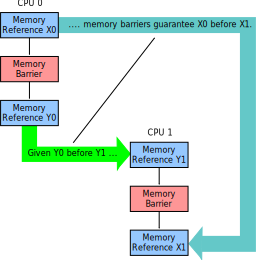
\includegraphics{memorder/memorybarrier}}
\caption{Memory Barriers Provide Conditional If-Then Ordering}
\label{fig:memorder:Memory Barriers Provide Conditional If-Then Ordering}
\end{figure}

\paragraph{Ordering has conditional if-then semantics.}
Figure~\ref{fig:memorder:Memory Barriers Provide Conditional If-Then Ordering}
illustrates this for memory barriers.
Assuming that both memory barriers are strong enough (and when in doubt, you
can always use \co{smp_mb()}), if CPU~1's access Y1 happens after CPU~0's
access Y0, then CPU~1's access X1 is guaranteed to happen after CPU~0's
access X1.

\QuickQuiz{}
	How can you tell which memory barriers are strong enough for
	a given use case?
\QuickQuizAnswer{
	Ah, that is a deep question whose answer requires most of the
	rest of this chapter.
} \QuickQuizEnd

Listing~\ref{lst:memorder:Memory Ordering: Store-Buffering Litmus Test}
is a case in point.
The \co{smp_mb()} on line~10 and~20 serve as the barriers,
the store to \co{x0} on line~9 as X0, the load from \co{x1} on line~11
as Y0, the store to \co{x1} on line~19 as Y1, and the load from
\co{x0} as X1.
Applying the if-then rule step by step, we know that the store to
\co{x1} on line~19 happens after the load from \co{x1} on line~11 if
\co{P0()}'s local variable \co{r2} is set to the value zero.
The if-then rule would then state that the load from \co{x0} on
line~21 happens after the store to \co{x0} on line~9.
In other words,
\co{P1()}'s local variable \co{r2} is guaranteed
to end up with the value two \emph{only if}
\co{P0()}'s local variable \co{r2} ends up with the value zero.
Again, memory ordering guarantees are conditional, not absolute.

Although
Figure~\ref{fig:memorder:Memory Barriers Provide Conditional If-Then Ordering}
specifically mentions memory barriers, the same rule applies to the
rest of the Linux kernel's ordering operations.

\paragraph{Ordering operations must be paired.}
If you carefully order the operations in one thread, but then fail to do
so in another thread, then there is no ordering.
Both threads must provide ordering for the if-then rule to apply.\footnote{
	In Section~\ref{sec:memorder:Propagation}, pairing will be
	generalized to cycles.}

\paragraph{Ordering operations almost never speed things up.}
If you find yourself tempted to add a memory barrier in an attempt
to force a prior store to be flushed to memory faster, resist!
Adding ordering usually slows things down.
Of course, there are situations where adding instructions speeds things
up, but careful benchmarking is required in such cases.
And even then, it is quite possible that although you sped things up
a little bit on \emph{your} system, you might well have slowed things
down significantly on your users' systems.
Or on your future system.

\paragraph{Ordering operations are not magic.}
When your program is failing due to some race condition, it is often
tempting to toss in a few memory-ordering operations in an attempt
to barrier your bug out of existence.
A far better reaction is to use higher-level primitives in a carefully
designed manner.
With concurrent programming, it is almost always easier to design
your bugs out of existence than to hack them out of existence!

\paragraph{These are only rough rules of thumb.}
Although these rules of thumb cover the vast majority of situations
seen in actual practice, as with any set of rules of thumb, they
do have their limits.
The next section will demonstrate some of these limits by introducing
trick-and-trap litmus tests that are intended to insult your
intuition while increasing your understanding.
These litmus tests will also illuminate many of the concepts
represented by the Linux-kernel memory-ordering cheat sheet shown in
Table~\ref{tab:memorder:Linux-Kernel Memory-Ordering Cheat Sheet}.
Section~\ref{sec:memorder:Where is Memory Ordering Needed?} will
circle back to this cheat sheet in light of learnings from all the
intervening tricks and traps.

\section{Tricks and Traps}
\label{sec:memorder:Tricks and Traps}

Now that you know that hardware can reorder memory accesses and that you
can prevent it from doing so, the next step is to get you to admit
that your intuition has a problem.
This painful task is taken up by
Section~\ref{sec:memorder:Variables With Multiple Values},
which presents some code demonstrating that scalar variables can
take on multiple values simultaneously,
and by
Sections~\ref{sec:memorder:Memory-Reference Reordering} through
\ref{sec:memorder:Multicopy Atomicity},
which show a series of intuitively correct code fragments that fail miserably
on real hardware.
Once your intuition has made it through the grieving process, later
sections will summarize the basic rules that memory ordering follows.

But first, let's take a quick look at just how many values a single
variable might have at a single moment of time.

\subsection{Variables With Multiple Values}
\label{sec:memorder:Variables With Multiple Values}

It is natural to think of a variable as taking on a well-defined
sequence of values in a well-defined, global order.
Unfortunately, the next stop on the journey says ``goodbye'' to this comforting fiction.
Hopefully, you already started to say ``goodbye'' in response to row~2 of
Tables~\ref{tab:memorder:Memory Misordering: Store-Buffering Sequence of Events}
and~\ref{tab:memorder:Memory Ordering: Store-Buffering Sequence of Events},
and if so, the purpose of this section is to drive this point home.

To this end, consider the program fragment shown in
Listing~\ref{lst:memorder:Software Logic Analyzer}.
This code fragment is executed in parallel by several CPUs.
Line~1 sets a shared variable to the current CPU's ID, line~2
initializes several variables from a \co{gettb()} function that
delivers the value of a fine-grained hardware ``timebase'' counter that is
synchronized among all CPUs (not available from all CPU architectures,
unfortunately!), and the loop from lines~3-8 records the length of
time that the variable retains the value that this CPU assigned to it.
Of course, one of the CPUs will ``win'', and would thus never exit
the loop if not for the check on lines~6-7.

\QuickQuiz{}
	What assumption is the code fragment
	in Listing~\ref{lst:memorder:Software Logic Analyzer}
	making that might not be valid on real hardware?
\QuickQuizAnswer{
	The code assumes that as soon as a given CPU stops
	seeing its own value, it will immediately see the
	final agreed-upon value.
	On real hardware, some of the CPUs might well see several
	intermediate results before converging on the final value.
	The actual code used to produce the data in the figures
	discussed later in this section was therefore somewhat more
	complex.
} \QuickQuizEnd

\begin{listing}[tbp]
{ \scriptsize
\begin{verbbox}
  1 state.variable = mycpu;
  2 lasttb = oldtb = firsttb = gettb();
  3 while (state.variable == mycpu) {
  4   lasttb = oldtb;
  5   oldtb = gettb();
  6   if (lasttb - firsttb > 1000)
  7     break;
  8 }
\end{verbbox}
}
\centering
\theverbbox
\caption{Software Logic Analyzer}
\label{lst:memorder:Software Logic Analyzer}
\end{listing}

Upon exit from the loop, \co{firsttb} will hold a timestamp
taken shortly after the assignment and \co{lasttb} will hold
a timestamp taken before the last sampling of the shared variable
that still retained the assigned value, or a value equal to \co{firsttb}
if the shared variable had changed before entry into the loop.
This allows us to plot each CPU's view of the value of \co{state.variable}
over a 532-nanosecond time period, as shown in
Figure~\ref{fig:memorder:A Variable With Multiple Simultaneous Values}.
This data was collected in 2006 on 1.5\,GHz POWER5 system with 8 cores,
each containing a pair of hardware threads.
CPUs~1, 2, 3, and~4 recorded the values, while CPU~0 controlled the test.
The timebase counter period was about 5.32\,ns, sufficiently fine-grained
to allow observations of intermediate cache states.

\begin{figure}[htb]
\centering
\resizebox{3in}{!}{\includegraphics{memorder/MoreThanOneValue}}
\caption{A Variable With Multiple Simultaneous Values}
\label{fig:memorder:A Variable With Multiple Simultaneous Values}
\end{figure}

Each horizontal bar represents the observations of a given CPU over time,
with the black regions to the left indicating the time before the
corresponding CPU's first measurement.
During the first 5\,ns, only CPU~3 has an opinion about the value of the
variable.
During the next 10\,ns, CPUs~2 and~3 disagree on the value of the variable,
but thereafter agree that the value is~``2'', which is in fact
the final agreed-upon value.
However, CPU~1 believes that the value is~``1'' for almost 300\,ns, and
CPU~4 believes that the value is~``4'' for almost 500\,ns.

\QuickQuiz{}
	How could CPUs possibly have different views of the
	value of a single variable \emph{at the same time?}
\QuickQuizAnswer{
	As discussed in
	Section~\ref{sec:memorder:Why Hardware Misordering?},
	many CPUs have store buffers that record the values of
	recent stores, which do not become globally visible until
	the corresponding cache line makes its way to the CPU.
	Therefore, it is quite possible for each CPU to see a
	different value for a given variable at a single point
	in time---and for main memory to hold yet another value.
	One of the reasons that memory barriers were invented was
	to allow software to deal gracefully with situations like
	this one.
} \QuickQuizEnd

\QuickQuiz{}
	Why do CPUs~2 and~3 come to agreement so quickly, when it
	takes so long for CPUs~1 and~4 to come to the party?
\QuickQuizAnswer{
	CPUs~2 and~3 are a pair of hardware threads on the same
	core, sharing the same cache hierarchy, and therefore have
	very low communications latencies.
	This is a NUMA, or, more accurately, a NUCA effect.

	This leads to the question of why CPUs~2 and~3 ever disagree
	at all.
	One possible reason is that they each might have a small amount
	of private cache in addition to a larger shared cache.
	Another possible reason is instruction reordering, given the
	short 10-nanosecond duration of the disagreement and the
	total lack of memory barriers in the code fragment.
} \QuickQuizEnd

And if you think that the situation with four CPUs was intriguing, consider
Figure~\ref{fig:memorder:A Variable With More Simultaneous Values},
which shows the same situation, but with 15~CPUs each assigning their
number to a single shared variable at time~$t=0$. Both diagrams in the
figure are drawn in the same way as 
Figure~\ref{fig:memorder:A Variable With Multiple Simultaneous Values}.
The only difference is that the unit of horizontal axis is timebase ticks,
with each tick lasting about 5.3~nanoseconds.
The entire sequence therefore lasts a bit longer than the events recorded in
Figure~\ref{fig:memorder:A Variable With Multiple Simultaneous Values},
consistent with the increase in number of CPUs.
The upper diagram shows the overall picture, while the lower one shows
the zoom-up of first 50~timebase ticks.

Again, CPU~0 coordinates the test, so does not record any values.

\begin{figure*}
\centering
\resizebox{5in}{!}{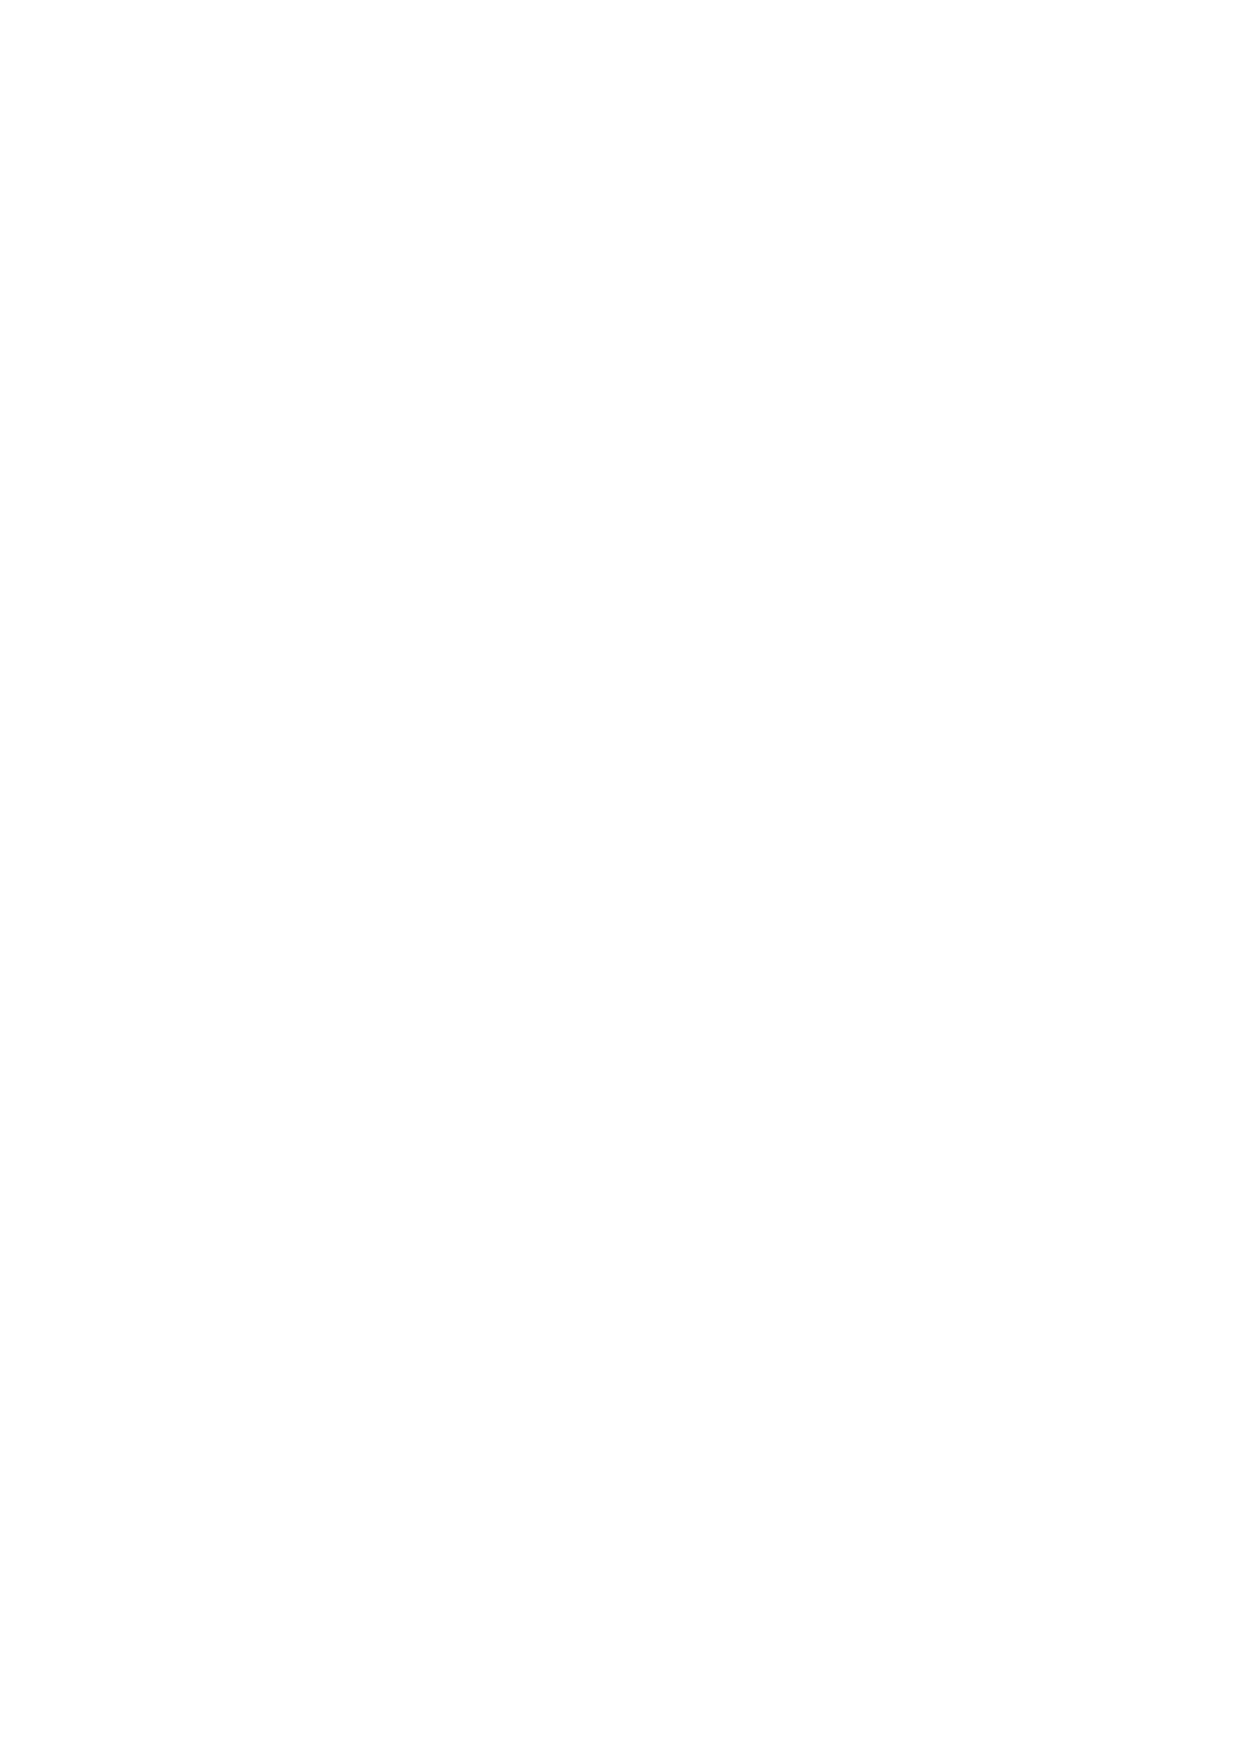
\includegraphics{memorder/MoreThanOneValue-15CPU}}
\caption{A Variable With More Simultaneous Values}
\ContributedBy{Figure}{fig:memorder:A Variable With More Simultaneous Values}{Akira Yokosawa}
\end{figure*}

All CPUs eventually agree on the final value of~9, but not before
the values~15 and~12 take early leads.
Note that there are fourteen different opinions on the variable's value
at time~21 indicated by the vertical line in the lower diagram.
Note also that all CPUs see sequences whose orderings are consistent with
the directed graph shown in
Figure~\ref{fig:memorder:Possible Global Orders With More Simultaneous Values}.
Nevertheless, both figures underscore the importance of
proper use of memory barriers for code that cares about memory ordering.

\begin{figure}[htb]
\centering
\resizebox{2.0in}{!}{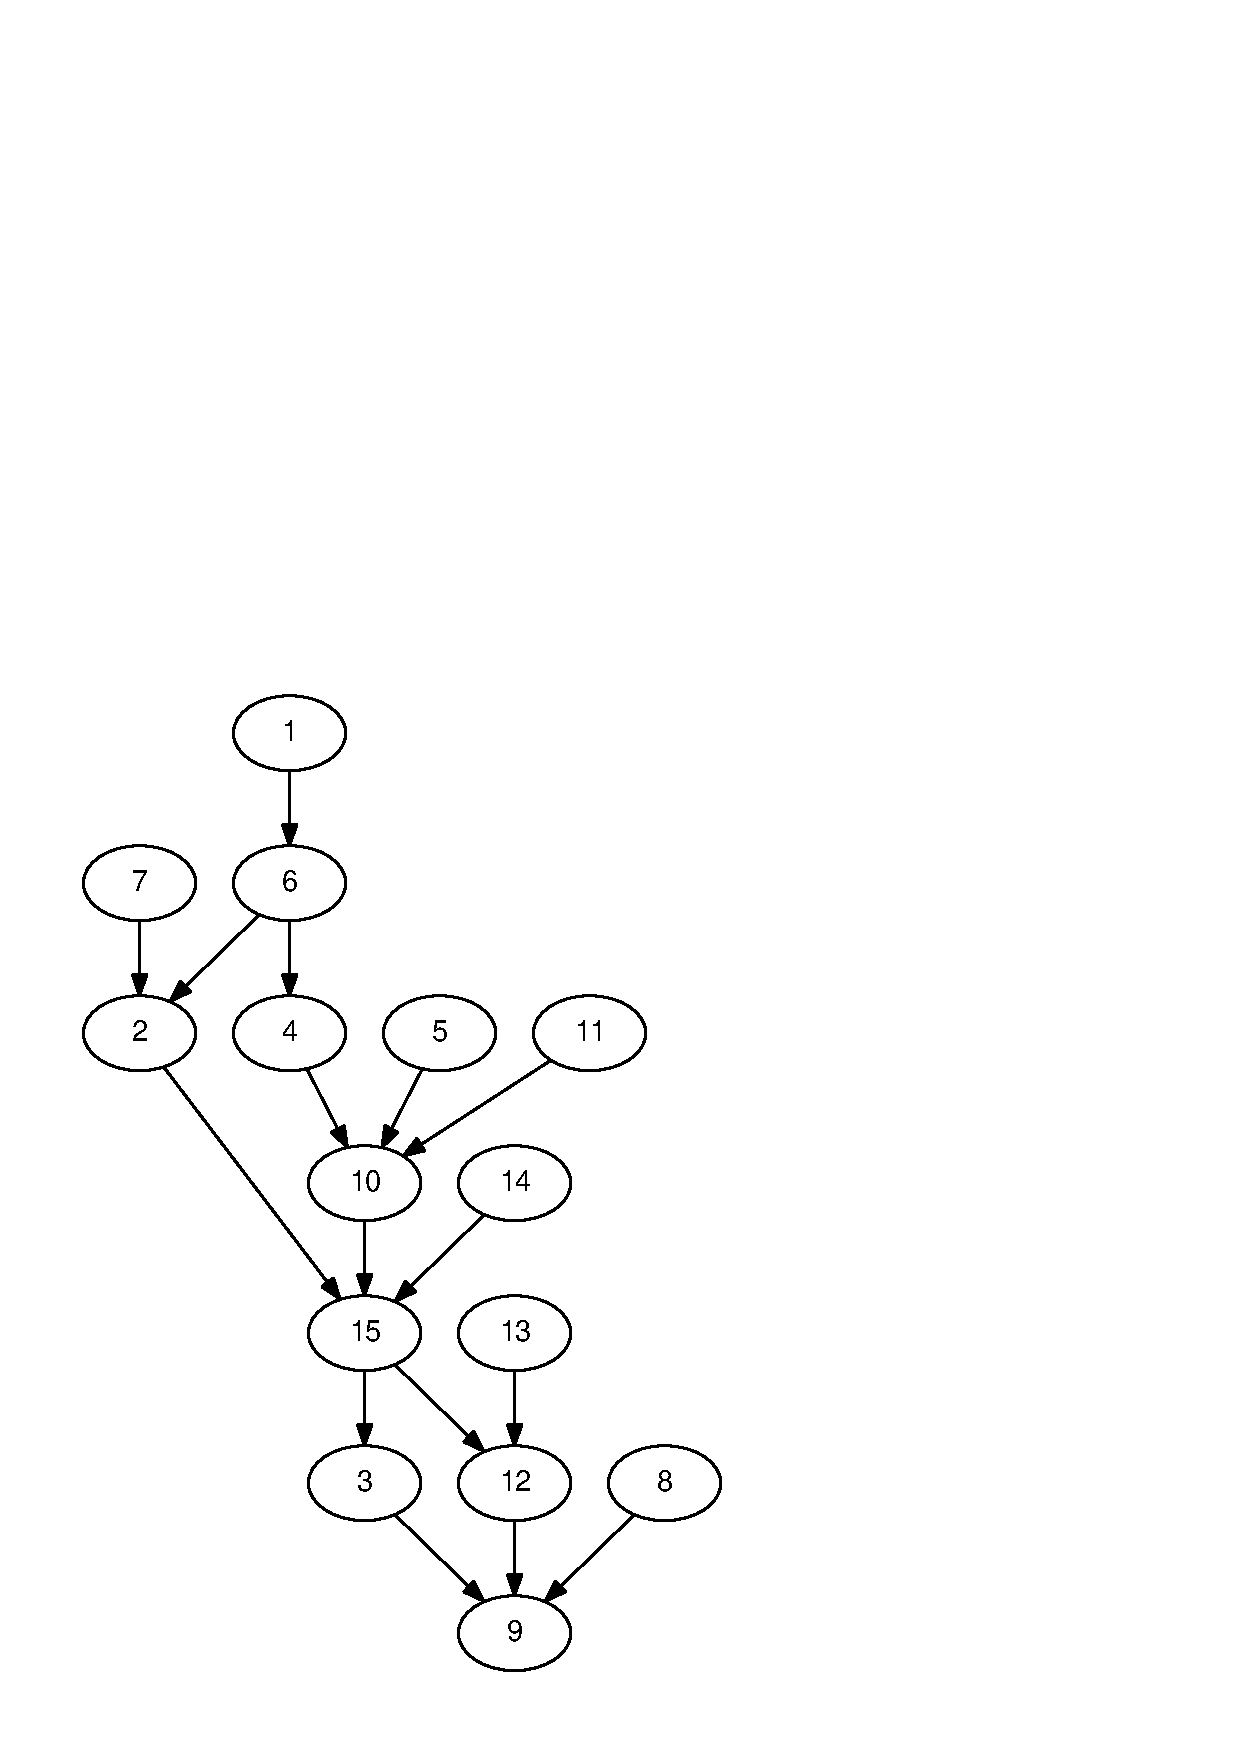
\includegraphics{memorder/store15tred}}
\caption{Possible Global Orders With More Simultaneous Values}
\label{fig:memorder:Possible Global Orders With More Simultaneous Values}
\end{figure}

How many values can a single variable take on at a single point in
time?
As many as one per store buffer in the system!
We have therefore entered a regime where we must bid a fond farewell to
comfortable intuitions about values of variables and the passage of time.
This is the regime where memory barriers are needed.

All that aside, it is important to remember the lessons from
Chapters~\ref{chp:Hardware and its Habits}
and~\ref{cha:Partitioning and Synchronization Design}.
Having all CPUs store concurrently to the same variable
is absolutely no way to design a parallel program, at least
not if performance and scalability are at all important to you.

Unfortunately, memory ordering has many other ways of insulting your
intuition, and not all of these ways conflict with performance and
scalability.
The next section will give an overview of reordering of unrelated
memory reference.

\subsection{Memory-Reference Reordering}
\label{sec:memorder:Memory-Reference Reordering}

Section~\ref{sec:memorder:Why Hardware Misordering?}
showed that even relatively strongly ordered systems like x86
can reorder prior stores with later loads, at least when the
store and load are to different variables.
This section builds on that result, looking at the other combinations of
loads and stores.

% @@@ Rationale for further reordering.

\begin{listing}[tbp]
{ \scriptsize
\begin{verbbox}[\LstLineNo]
C C-MP+o-wmb-o+o-o

{
}


P0(int* x0, int* x1) {

  WRITE_ONCE(*x0, 2);
  smp_wmb();
  WRITE_ONCE(*x1, 2);

}

P1(int* x0, int* x1) {

  int r2;
  int r3;

  r2 = READ_ONCE(*x1);
  r3 = READ_ONCE(*x0);

}

exists (1:r2=2 /\ 1:r3=0)
\end{verbbox}
}
\centering
\theverbbox
\caption{Message-Passing Litmus Test (No Ordering)}
\label{lst:memorder:Message-Passing Litmus Test (No Ordering)}
\end{listing}

\subsubsection{Load Followed By Load}
Listing~\ref{lst:memorder:Message-Passing Litmus Test (No Ordering)}
(\path{C-MP+o-wmb-o+o-o.litmus})
shows the classic \emph{message-passing} litmus test, where \co{x0} is
the message and \co{x1} is a flag indicating whether or not a message
is available.
In this test, the \co{smp_wmb()} forces \co{P0()} stores to be ordered,
but no ordering is specified for the loads.
Relatively strongly ordered architectures, such as x86, do enforce ordering.
However, weakly ordered architectures often do
not~\cite{JadeAlglave2011ppcmem}.
Therefore, the \co{exists} clause on line~25 of the listing \emph{can}
trigger.

\begin{listing}[tbp]
{ \scriptsize
\begin{verbbox}[\LstLineNo]
C C-MP+o-wmb-o+o-rmb-o

{
}

P0(int* x0, int* x1) {

  WRITE_ONCE(*x0, 2);
  smp_wmb();
  WRITE_ONCE(*x1, 2);

}

P1(int* x0, int* x1) {

  int r2;
  int r3;

  r2 = READ_ONCE(*x1);
  smp_rmb();
  r3 = READ_ONCE(*x0);

}

exists (1:r2=2 /\ 1:r3=0)
\end{verbbox}
}
\centering
\theverbbox
\caption{Enforcing Order of Message-Passing Litmus Test}
\label{lst:memorder:Enforcing Order of Message-Passing Litmus Test}
\end{listing}

Thus, portable code relying on ordering in this case must
add explicit ordering, for example, the \co{smp_rmb()} shown on
line~20 of
Listing~\ref{lst:memorder:Enforcing Order of Message-Passing Litmus Test}
(\path{C-MP+o-wmb-o+o-rmb-o.litmus}), which prevents
the \co{exists} clause from triggering.

\begin{listing}[tbp]
{ \scriptsize
\begin{verbbox}[\LstLineNo]
C C-LB+o-o+o-o
{
}

P0(int *x0, int *x1)
{
  int r2;

  r2 = READ_ONCE(*x1);
  WRITE_ONCE(*x0, 2);
}


P1(int *x0, int *x1)
{
  int r2;

  r2 = READ_ONCE(*x0);
  WRITE_ONCE(*x1, 2);
}

exists (1:r2=2 /\ 0:r2=2)
\end{verbbox}
}
\centering
\theverbbox
\caption{Load-Buffering Litmus Test (No Ordering)}
\label{lst:memorder:Load-Buffering Litmus Test (No Ordering)}
\end{listing}

\subsubsection{Load Followed By Store}
Listing~\ref{lst:memorder:Load-Buffering Litmus Test (No Ordering)}
(\path{C-LB+o-o+o-o.litmus})
shows the classic \emph{load-buffering} litmus test.
Although relatively strongly ordered systems such as x86
or the IBM Mainframe do not reorder prior loads with subsequent stores,
more weakly ordered architectures really do allow such
reordering~\cite{JadeAlglave2011ppcmem}.
Therefore, the \co{exists} clause on line~22 really can trigger.

\begin{listing}[tbp]
{ \scriptsize
\begin{verbbox}[\LstLineNo]
C C-LB+o-r+a-o
{
}

P0(int *x0, int *x1)
{
  int r2;

  r2 = READ_ONCE(*x1);
  smp_store_release(x0, 2);
}


P1(int *x0, int *x1)
{
  int r2;

  r2 = smp_load_acquire(x0);
  WRITE_ONCE(*x1, 2);
}

exists (1:r2=2 /\ 0:r2=2)
\end{verbbox}
}
\centering
\theverbbox
\caption{Enforcing Ordering of Load-Buffering Litmus Test}
\label{lst:memorder:Enforcing Ordering of Load-Buffering Litmus Test}
\end{listing}

Although it is rare for actual hardware to
exhibit this reordering~\cite{LucMaranget2017aarch64},
portable code must nevertheless enforce any required ordering, for example,
as shown in
Listing~\ref{lst:memorder:Enforcing Ordering of Load-Buffering Litmus Test}
(\path{C-LB+o-r+a-o.litmus}).
This guarantees that the \co{exists} clause on line~22 never triggers.

\begin{listing}[tbp]
{ \scriptsize
\begin{verbbox}[\LstLineNo]
C C-MP+o-o+o-rmb-o

{
}

P0(int* x0, int* x1) {

  WRITE_ONCE(*x0, 2);
  WRITE_ONCE(*x1, 2);

}

P1(int* x0, int* x1) {

  int r2;
  int r3;

  r2 = READ_ONCE(*x1);
  smp_rmb();
  r3 = READ_ONCE(*x0);

}

exists (1:r2=2 /\ 1:r3=0)
\end{verbbox}
}
\centering
\theverbbox
\caption{Message-Passing Litmus Test, No Writer Ordering (No Ordering)}
\label{lst:memorder:Message-Passing Litmus Test, No Writer Ordering (No Ordering)}
\end{listing}

\subsubsection{Store Followed By Store}
Listing~\ref{lst:memorder:Message-Passing Litmus Test, No Writer Ordering (No Ordering)}
(\path{C-MP+o-o+o-rmb-o.litmus})
once again shows the classic message-passing litmus test, but without
explicit ordering for \co{P0()}'s stores and with the \co{smp_rmb()}
providing ordering for \co{P1()}'s loads.
Again, the relatively strongly ordered architectures do enforce ordering,
but weakly ordered architectures do not necessarily do
so~\cite{JadeAlglave2011ppcmem}, which means that the
\co{exists} clause can trigger.
Therefore, portable code must explicitly order the stores, for
example, as shown in
Listing~\ref{lst:memorder:Enforcing Order of Message-Passing Litmus Test},
thus preventing the \co{exists} clause from triggering.

\subsection{Address Dependencies}
\label{sec:memorder:Address Dependencies}

An \emph{address dependency} occurs when the value returned by a load
instruction is used to compute the address used by a later memory-reference
instruction.

\begin{listing}[tbp]
{ \scriptsize
\begin{verbbox}[\LstLineNo]
C C-MP+o-wmb-o+o-addr-o

{
int y=1;
int *x1 = &y;
}

P0(int* x0, int** x1) {

  WRITE_ONCE(*x0, 2);
  smp_wmb();
  WRITE_ONCE(*x1, x0);

}

P1(int** x1) {

  int *r2;
  int r3;

  r2 = READ_ONCE(*x1);
  r3 = READ_ONCE(*r2);

}

exists (1:r2=x0 /\ 1:r3=1)
\end{verbbox}
}
\centering
\theverbbox
\caption{Message-Passing Address-Dependency Litmus Test (No Ordering)}
\label{lst:memorder:Message-Passing Address-Dependency Litmus Test (No Ordering)}
\end{listing}

Listing~\ref{lst:memorder:Message-Passing Address-Dependency Litmus Test (No Ordering)}
(\path{C-MP+o-wmb-o+o-addr-o.litmus})
shows a linked variant of the message-passing pattern.
The head pointer is \co{x1}, which initially
references the \co{int} variable \co{y} (line~5), which is in turn 
initialized to the value $1$ (line~4).
\co{P0()} updates head pointer \co{x1} to reference \co{x0} (line~12),
but only afer initializing it to $2$ (line~10) and forcing ordering
(line~11).
\co{P1()} picks up the head pointer \co{x1} (line~21), and then loads
the referenced value (line~22).
There is thus an address dependency from the load on line~21 to the
load on line~22.
In this case, the value returned by line~21 is exactly the address
used by line~22, but many variations are possible,
including field access using the C-language \co{->} operator,
addition, subtraction, and array indexing.

One might hope that line~21's load from the head pointer would be ordered
before line~22's dereference.
However, this is not the case on DEC Alpha, which can in effect use
a speculated value for the dependent load, as described in more detail in
Section~\ref{sec:app:whymb:Alpha}.
Therefore,
Listing~\ref{lst:memorder:Message-Passing Address-Dependency Litmus Test (No Ordering)}'s
\co{exists} clause \emph{can} trigger.

\begin{listing}[tbp]
{ \scriptsize
\begin{verbbox}[\LstLineNo]
C C-MP+o-wmb-o+ld-addr-o

{
int y=1;
int *x1 = &y;
}

P0(int* x0, int** x1) {

  WRITE_ONCE(*x0, 2);
  smp_wmb();
  WRITE_ONCE(*x1, x0);

}

P1(int** x1) {

  int *r2;
  int r3;

  r2 = lockless_dereference(*x1);
  r3 = READ_ONCE(*r2);

}

exists (1:r2=x0 /\ 1:r3=1)
\end{verbbox}
}
\centering
\theverbbox
\caption{Enforced Ordering of Message-Passing Address-Dependency Litmus Test}
\label{lst:memorder:Enforced Ordering of Message-Passing Address-Dependency Litmus Test}
\end{listing}

Listing~\ref{lst:memorder:Enforced Ordering of Message-Passing Address-Dependency Litmus Test}
(\path{C-MP+o-wmb-o+ld-addr-o.litmus})
shows how to make this work portably, even on DEC Alpha, by
replacing line~21's \co{READ_ONCE()} with \co{lockless_dereference()},
which acts like \co{READ_ONCE()} on all platforms other than DEC Alpha,
where it acts like a \co{READ_ONCE()} followed by an \co{smp_mb()},
thereby forcing the required ordering on all platforms, in turn
preventing the \co{exists} clause from triggering.

\begin{listing}[tbp]
{ \scriptsize
\begin{verbbox}[\LstLineNo]
C C-S+o-wmb-o+o-addr-o

{
int y=1;
int *x1 = &y;
}

P0(int* x0, int** x1) {

  WRITE_ONCE(*x0, 2);
  smp_wmb();
  WRITE_ONCE(*x1, x0);

}

P1(int** x1) {

  int *r2;

  r2 = READ_ONCE(*x1);
  WRITE_ONCE(*r2, 3);

}

exists (1:r2=x0 /\ x0=2)
\end{verbbox}
}
\centering
\theverbbox
\caption{S Address-Dependency Litmus Test}
\label{lst:memorder:S Address-Dependency Litmus Test}
\end{listing}

But what happens if the dependent operation is a store rather than
a load, for example, in the \emph{S}
litmus test~\cite{JadeAlglave2011ppcmem} shown in
Listing~\ref{lst:memorder:S Address-Dependency Litmus Test}
(\path{C-S+o-wmb-o+o-addr-o.litmus})?
Because no production-quality platform speculates stores,
it is not possible for the \co{WRITE_ONCE()} on line~10 to overwrite
the \co{WRITE_ONCE()} on line~21, meaning that the \co{exists}
clause on line~25 cannot trigger, even on DEC Alpha, even
without the \co{lockless_dereference()} that is required in the
dependent-load case.

\QuickQuiz{}
	But how do we know that \emph{all} platforms really avoid
	triggering the \co{exists} clauses in
	Listings~\ref{lst:memorder:Enforced Ordering of Message-Passing Address-Dependency Litmus Test}
	and~\ref{lst:memorder:S Address-Dependency Litmus Test}?
\QuickQuizAnswer{
	Answering this requires identifying three major groups of platforms:
	(1)~Total-store-order (TSO) platforms,
	(2)~Weakly ordered platorms, and
	(3)~DEC Alpha.

	The TSO platforms order all pairs of memory references except for
	prior stores against later loads.
	Because the address dependency on lines~21 and~22 of
	Listing~\ref{lst:memorder:Enforced Ordering of Message-Passing Address-Dependency Litmus Test}
	is instead a load followed by another load, TSO platforms preserve
	this address dependency.
	They also preserve the address dependency on lines~20 and~21 of
	Listing~\ref{lst:memorder:S Address-Dependency Litmus Test}
	because this is a load followed by a store.
	Because address dependencies must start with a load, TSO platforms
	implicitly but completely respect them.

	Weakly ordered platforms don't necessarily maintain ordering of
	unrelated accesses.
	However, the address dependencies in
	Listings~\ref{lst:memorder:Enforced Ordering of Message-Passing Address-Dependency Litmus Test}
	and~\ref{lst:memorder:S Address-Dependency Litmus Test}
	are not unrelated: There is an address dependency.
	The hardware tracks dependencies and maintains the needed
	ordering.

	There is one (famous) exception to this rule for weakly ordered
	platforms, and that exception is DEC Alpha for load-to-load
	address dependencies.
	And this is why DEC Alpha requires the explicit memory barrier
	supplied for it by the \co{lockless_dereference()} on line~21 of
	Listings~\ref{lst:memorder:Enforced Ordering of Message-Passing Address-Dependency Litmus Test}.
	However, DEC Alpha does track load-to-store address dependencies,
	which is why line~20 of
	Listings~\ref{lst:memorder:S Address-Dependency Litmus Test}
	does not have a \co{lockless_dereference()}.

	To sum up, current platforms either respect address dependencies
	implicitly, as is the case for TSO platforms (x86, mainframe,
	SPARC,~...), have hardware tracking for address dependencies
	(ARM, PowerPC, MIPS,~...), or have the required memory barriers
	supplied by \co{lockless_dereference()} (DEC Alpha).
} \QuickQuizEnd

However, it is important to note that address dependencies can
be fragile and easily broken by compiler optimizations, as discussed in
Section~\ref{sec:memorder:Address- and Data-Dependency Restrictions}.

\subsection{Data Dependencies}
\label{sec:memorder:Data Reordering}

A \emph{data dependency} occurs when the value returned by a load
instruction is used to compute the data stored by a later store
instruction.
Note well the ``data'' above: If the value returned by a load
was instead used to compute the address used by a later store
instruction, that would instead be an address dependency.

\begin{listing}[tbp]
{ \scriptsize
\begin{verbbox}[\LstLineNo]
C C-LB+o-r+o-data-o
{
}

P0(int *x0, int *x1)
{
  int r2;

  r2 = READ_ONCE(*x1);
  smp_store_release(x0, 2);
}


P1(int *x0, int *x1)
{
  int r2;

  r2 = READ_ONCE(*x0);
  WRITE_ONCE(*x1, r2);
}

exists (1:r2=2 /\ 0:r2=2)
\end{verbbox}
}
\centering
\theverbbox
\caption{Load-Buffering Data-Dependency Litmus Test}
\label{lst:memorder:Load-Buffering Data-Dependency Litmus Test}
\end{listing}

Listing~\ref{lst:memorder:Load-Buffering Data-Dependency Litmus Test}
(\path{C-LB+o-r+o-data-o.litmus})
is similar to
Listing~\ref{lst:memorder:Enforcing Ordering of Load-Buffering Litmus Test},
except that \co{P1()}'s ordering between lines~18 and~19 is
enforced not by an acquire load, but instead by a data dependency:
The value loaded by line~18 is what line~19 stores.
The ordering provided by this data dependency is sufficient to prevent
the \co{exists} clause from triggering.

\QuickQuiz{}
	Why doesn't line~18 of
	Listing~\ref{lst:memorder:Load-Buffering Data-Dependency Litmus Test}
	need a \co{lockless_dereference()}?
\QuickQuizAnswer{
	Data dependencies are always load-to-store dependencies, and
	so all platforms respect them, even DEC Alpha, and for the
	same reasons that they respect load-to-store address dependencies.
} \QuickQuizEnd

Just as with address dependencies, data dependencies are
fragile and can be easily broken by compiler optimizations, as discussed in
Section~\ref{sec:memorder:Address- and Data-Dependency Restrictions}.
In fact, data dependencies can be even more fragile than are address
dependencies.
The reason for this is that address dependencies normally involve
pointer values.
In contrast, as shown in
Listing~\ref{lst:memorder:Load-Buffering Data-Dependency Litmus Test},
it is tempting to carry data dependencies through integral values,
which the compiler has much more freedom to optimize into nonexistence.
For but one example, if the integer loaded was multiplied by the constant
zero, the compiler would know that the result was zero, and could therefore
substitute the constant zero for the value loaded, thus breaking
the dependency.

\QuickQuiz{}
	But wait!!!
	Line~18 of
	Listing~\ref{lst:memorder:Load-Buffering Data-Dependency Litmus Test}
	uses \co{READ_ONCE()}, which marks the load as volatile,
	which means that the compiler absolutely must emit the load
	instruction even if the value is later multiplied by zero.
	So do you really need to work so hard to keep the compiler from
	breaking your data dependencies?
\QuickQuizAnswer{
	Yes, the compiler absolutely must emit a load instruction for
	a volatile load.
	But if you multiply the value loaded by zero, the compiler is
	well within its rights to substitute a constant zero for the
	result of that multiplication, which will break the data
	dependency on many platforms.

	Worse yet, if the dependent store does not use \co{WRITE_ONCE()},
	the compiler could hoist it above the load, which would cause
	even TSO platforms to fail to provide ordering.
} \QuickQuizEnd

In short, you can rely on data dependencies, but only if you take care
to prevent your compiler from breaking them.

\subsection{Control Dependencies}
\label{sec:memorder:Control Dependencies}

A \emph{control dependency} occurs when the value returned by a load
instruction is tested to determine whether or not a later store instruction
is executed.
Note well the ``later store instruction'': Many platforms do not respect
load-to-load control dependencies.

\begin{listing}[tbp]
{ \scriptsize
\begin{verbbox}[\LstLineNo]
C C-LB+o-r+o-ctrl-o
{
}

P0(int *x0, int *x1)
{
  int r2;

  r2 = READ_ONCE(*x1);
  smp_store_release(x0, 2);
}


P1(int *x0, int *x1)
{
  int r2;

  r2 = READ_ONCE(*x0);
  if (r2 >= 0)
    WRITE_ONCE(*x1, 2);
}

exists (1:r2=2 /\ 0:r2=2)
\end{verbbox}
}
\centering
\theverbbox
\caption{Load-Buffering Control-Dependency Litmus Test}
\label{lst:memorder:Load-Buffering Control-Dependency Litmus Test}
\end{listing}

Listing~\ref{lst:memorder:Load-Buffering Control-Dependency Litmus Test}
(\path{C-LB+o-r+o-ctrl-o.litmus})
shows another load-buffering example, this time using a control
dependency (line~19) to order the load on line~18 and the store on
line~20.
The ordering is sufficient to prevent the \co{exists} from triggering.

However, control dependencies are even more susceptible to being optimized
out of existence than are data dependencies, and
Section~\ref{sec:memorder:Control-Dependency Restrictions}
describes some of the rules that must be followed in order to prevent
your compiler from breaking your control dependencies.

\begin{listing}[tbp]
{ \scriptsize
\begin{verbbox}[\LstLineNo]
C C-MP+o-r+o-ctrl-o

{
}

P0(int* x0, int* x1) {

  WRITE_ONCE(*x0, 2);
  smp_store_release(x1, 2);

}

P1(int* x0, int* x1) {
  int r2;
  int r3 = 0;

  r2 = READ_ONCE(*x1);
  if (r2 >= 0)
    r3 = READ_ONCE(*x0);

}

exists (1:r2=2 /\ 1:r3=0)
\end{verbbox}
}
\centering
\theverbbox
\caption{Message-Passing Control-Dependency Litmus Test (No Ordering)}
\label{lst:memorder:Message-Passing Control-Dependency Litmus Test (No Ordering)}
\end{listing}

It is worth reiterating that control dependencies provide ordering only
from loads to stores.
Therefore, the load-to-load control dependency shown on lines~17-19 of
Listing~\ref{lst:memorder:Message-Passing Control-Dependency Litmus Test (No Ordering)}
(\path{C-MP+o-r+o-ctrl-o.litmus})
does \emph{not} provide ordering, and therefore does \emph{not}
prevent the \co{exists} clause from triggering.

In summary, control dependencies can be useful, but they are
high-maintenance items.
You should therefore use them only when performance considerations
permit no other solution.

\QuickQuiz{}
	Wouldn't control dependencies be more robust if they were
	mandated by language standards???
\QuickQuizAnswer{
	In the fullness of time, perhaps they will be so mandated.
} \QuickQuizEnd

\subsection{Cache Coherence}
\label{sec:memorder:Cache Coherence}

On cache-coherent platforms, all CPUs agree on the order of loads and
stores to a given variable.
Fortunately, when \co{READ_ONCE()} and \co{WRITE_ONCE()} are used,
almost all platforms are cache-coherent, as indicated by the ``SV''
column of the cheat sheet shown in
Table~\ref{tab:memorder:Linux-Kernel Memory-Ordering Cheat Sheet}.
Unfortunately, this property is so popular that it has been named
multiple times, with ``single-variable SC'',\footnote{
	Recall that SC stands for sequentially consistent.}
``single-copy atomic''~\cite{Stone:1995:SP:623262.623912},
and just plain ``coherence''~\cite{JadeAlglave2011ppcmem}
having seen use.
Rather than further compound the confusion by inventing yet another term
for this concept, this book uses ``cache coherence'' and ``coherence''
interchangeably.

\begin{listing}[tbp]
{ \scriptsize
\begin{verbbox}[\LstLineNo]
C C-CCIRIW+o+o+o-o+o-o

{
int x = 0;
}

P0(int *x)
{
  WRITE_ONCE(*x, 1);
}

P1(int *x)
{
  WRITE_ONCE(*x, 2);
}

P2(int *x)
{
  int r1;
  int r2;

  r1 = READ_ONCE(*x);
  r2 = READ_ONCE(*x);
}

P3(int *x)
{
  int r3;
  int r4;

  r3 = READ_ONCE(*x);
  r4 = READ_ONCE(*x);
}

exists(2:r1=1 /\ 2:r2=2 /\ 3:r3=2 /\ 3:r4=1)
\end{verbbox}
}
\centering
\theverbbox
\caption{Cache-Coherent IRIW Litmus Test}
\label{lst:memorder:Cache-Coherent IRIW Litmus Test}
\end{listing}

Listing~\ref{lst:memorder:Cache-Coherent IRIW Litmus Test}
(\path{C-CCIRIW+o+o+o-o+o-o.litmus})
shows a litmus test that tests for cache coherence,
where ``IRIW'' stands
for ``independent reads of independent writes''.
Because this litmus test uses only one variable,
\co{P2()} and \co{P3()} must agree
on the order of \co{P0()}'s and \co{P1()}'s stores.
In other words, if \co{P2()} believes that \co{P0()}'s store
came first, then \co{P3()} had better not believe that
\co{P1()}'s store came first.
And in fact the \co{exists} clause on line~35 will trigger if this
situation arises.

It is tempting to speculate that different-sized overlapping loads 
and stores to a single region of memory (as might be set up using
the C-language \co{union} keyword) would provide similar ordering
guarantees.
However, Flur et al.~discovered some surprisingly simple
litmus tests that demonstrate that these guarantees can be violated on
real hardware~\cite{Flur:2017:MCA:3093333.3009839}.
It is therefore necessary to restrict code to non-overlapping
same-sized aligned accesses to a given variable, at least if portability
is a consideration.\footnote{
	There is reason to believe that using atomic RMW operations
	(for example, \co{xchg()}) for all the stores will
	provide sequentially consistent ordering, but this has not
	yet been proven either way.}

Adding more variables and threads increases the scope for reordering
and other counterintuitive behavior, as discussed in the next section.

\subsection{Multicopy Atomicity}
\label{sec:memorder:Multicopy Atomicity}

\begin{figure}[tb]
\centering
\resizebox{3.0in}{!}{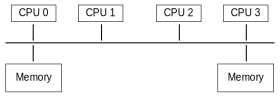
\includegraphics{memorder/SystemArchBus}}
\caption{Global System Bus And Multi-Copy Atomicity}
\label{fig:memorder:Global System Bus And Multi-Copy Atomicity}
\end{figure}

Threads running on a \emph{multicopy atomic}~\cite{Stone:1995:SP:623262.623912}
platform are guaranteed
to agree on the order of stores, even to different variables.
A useful mental model of such a system is the single-bus architecture
shown in
Figure~\ref{fig:memorder:Global System Bus And Multi-Copy Atomicity}.
If each store resulted in a message on the bus, and if the bus could
accommodate only one store at a time, then any pair of CPUs would
agree on the order of all stores that they observed.
Unfortunately, building a computer system as shown in the figure,
without store buffers or even caches, would result in glacial computation.
CPU vendors interested in providing multicopy atomicity have therefore
instead provided the slightly weaker
\emph{other-multicopy atomicity}~\cite[Section B2.3]{ARMv8A:2017},
which excludes the CPU doing a given store from the requirement that all
CPUs agree on the order of all stores.
This means that if only a subset of CPUs are doing stores, the
other CPUs will agree on the order of stores, hence the ``other''
in ``other-multicopy atomicity''.
Unlike multicopy-atomic platforms, within other-multicopy-atomic platforms,
the CPU doing the store is permitted to observe its
store early, which allows its later loads to obtain the newly stored
value directly from the store buffer.
This in turn avoids abysmal performance.

\QuickQuiz{}
	Can you give a specific example showing different behavior for
	multicopy atomic on the one hand and other-multicopy atomic
	on the other?
\QuickQuizAnswer{
\begin{listing}[tbp]
{ \scriptsize
\begin{verbbox}[\LstLineNo]
C C-MP-OMCA+o-o-o+o-rmb-o

{
}

P0(int *x, int *y)
{
  int r0;

  WRITE_ONCE(*x, 1);
  r0 = READ_ONCE(*x);
  WRITE_ONCE(*y, r0);
}

P1(int *x, int *y)
{
  int r1;
  int r2;

  r1 = READ_ONCE(*y);
  smp_rmb();
  r2 = READ_ONCE(*x);
}

exists (1:r1=1 /\ 1:r2=0)
\end{verbbox}
}
\centering
\theverbbox
\caption{Litmus Test Distinguishing Multicopy Atomic From Other Multicopy Atomic}
\label{lst:memorder:Litmus Test Distinguishing Multicopy Atomic From Other Multicopy Atomic}
\end{listing}

	Listing~\ref{lst:memorder:Litmus Test Distinguishing Multicopy Atomic From Other Multicopy Atomic}
	(\path{C-MP-OMCA+o-o-o+o-rmb-o.litmus})
	shows such a test.

	On a multicopy-atomic platform, \co{P0()}'s store to \co{x} on
	line~10 must become visible to both \co{P0()} and \co{P1()}
	simultaneously.
	Because this store becomes visible to \co{P0()} on line~11, before
	\co{P0()}'s store to \co{y} on line~12, \co{P0()}'s store to
	\co{x} must become visible before its store to \co{y} everywhere,
	including \co{P1()}.
	Therefore, if \co{P1()}'s load from \co{y} on line~20 returns the
	value 1, so must its load from \co{x} on line~22, given that
	the \co{smp_rmb()} on line~21 forces these two loads to execute
	in order.
	Therefore, the \co{exists} clause on line~25 cannot trigger on a
	multicopy-atomic platform.

	In contrast, on an other-multicopy-atomic platform, \co{P0()}
	could see its own store early, so that there would be no constraint
	on the order of visibility of the two stores from to \co{P1()},
	which in turn allows the \co{exists} clause to trigger.
} \QuickQuizEnd

Perhaps there will come a day when all platforms provide some flavor
of multi-copy atomicity, but
in the meantime, non-multicopy-atomic platforms do exist, and so software
does need to deal with them.

\begin{listing}[tbp]
{ \scriptsize
\begin{verbbox}[\LstLineNo]
C C-WWC+o+o-data-o+o-addr-o

{
int a = 0;
int b = 0;
int *c = &b;
int *x = &a;
int *y = &b;
}

P0(int **x)
{
  WRITE_ONCE(*x, x);
}

P1(int **x, int **y)
{
  int *r1;

  r1 = READ_ONCE(*x);
  WRITE_ONCE(*y, r1);
}

P2(int **y, int **c)
{
  int *r2;

  r2 = READ_ONCE(*y);
  WRITE_ONCE(*r2, c);
}

exists(1:r1=x /\ 2:r2=x /\ x=x)
\end{verbbox}
}
\centering
\theverbbox
\caption{WWC Litmus Test With Dependencies (No Ordering)}
\label{lst:memorder:WWC Litmus Test With Dependencies (No Ordering)}
\end{listing}

Listing~\ref{lst:memorder:WWC Litmus Test With Dependencies (No Ordering)}
(\path{C-WWC+o+o-data-o+o-addr-o.litmus})
demonstrates multicopy atomicity, that is, on a multicopy-atomic platform,
the \co{exists} clause on line~32 cannot trigger.
In contrast, on a non-multicopy-atomic
platform this \co{exists} clause can trigger, despite
\co{P1()}'s accesses being ordered by a data dependency and \co{P2()}'s
accesses being ordered by an address dependency.
Recall that the definition of multicopy atomicity requires that all
threads agree on the order of stores, which can be thought of as
all stores reaching all threads at the same time.
Therefore, a non-multicopy-atomic platform can have a store reach
different threads at different times.
In particular, \co{P0()}'s store might reach \co{P1()} long before it
reaches \co{P2()}, which raises the possibility that \co{P1()}'s store
might reach \co{P2()} before \co{P0()}'s store does.

\begin{figure}[tb]
\centering
\resizebox{3.0in}{!}{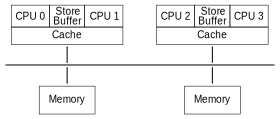
\includegraphics{memorder/NonMCAplatform}}
\caption{Shared Store Buffers And Multi-Copy Atomicity}
\label{fig:memorder:Shared Store Buffers And Multi-Copy Atomicity}
\end{figure}

This leads to the question of why a real system constrained by the
usual laws of physics would ever trigger the \co{exists} clause of
Listing~\ref{lst:memorder:WWC Litmus Test With Dependencies (No Ordering)}.
The cartoonish diagram of a such a real system is shown in
Figure~\ref{fig:memorder:Shared Store Buffers And Multi-Copy Atomicity}.
CPU~0 and CPU~1 share a store buffer, as do CPUs~2 and~3.
This means that CPU~1 can load a value out of the store buffer, thus
potentially immediately seeing a value stored by CPU~0.
In contrast, CPUs~2 and~3 will have to wait for the corresponding cache
line to carry this new value to them.

\QuickQuiz{}
	Then who would even \emph{think} of designing a system with shared
	store buffers???
\QuickQuizAnswer{
	This is in fact a very natural design for any system having
	multiple hardware threads per core.
	Natural from a hardware point of view, that is!
} \QuickQuizEnd

\begin{table*}
\small
\centering\OneColumnHSpace{-0.8in}
\begin{tabular}{r||l|l|l|l||l|l|l}
	& \tco{P0()} & \multicolumn{2}{c|}{\tco{P0()} \& \tco{P1()}} & \tco{P1()} & \multicolumn{3}{c}{\tco{P2()}} \\
	\cline{2-8}
	& Instruction & Store Buffer & Cache & Instruction &
			Instruction & Store Buffer & Cache \\
	\hline
	\hline
	1 & (Initial state) & & \tco{y==&b} &
		(Initial state) &
			(Initial state) & & \tco{x==&a} \\
	\hline
	2 & \tco{x = &x;} & \tco{x==&x} & \tco{y==&b} &
		 & & & \tco{x==&a} \\
	\hline
	3 & (Read-Invalidate \tco{x}) & \tco{x==&x} & \tco{y==&b} & \tco{r1 = x} (\tco{&x})
		 & & & \tco{x==&a} \\
	\hline
	4 &  & \tco{x==&x} \tco{y==&x} & \tco{y==&b} & \tco{y = r1}
		 & \tco{r2 = y} & & \tco{x==&a} \\
	\hline
	5 &  & \tco{x==&x} & \tco{y==&x} & (Finish store)
		 & (Read \tco{y}) & & \tco{x==&a} \\
	\hline
	6 & & \tco{x==&x} & \tco{y==&x} &
		 & (\tco{r2==&x}) & & \tco{x==&a} \tco{y==&x} \\
	\hline
	7 & & \tco{x==&x} & \tco{y==&x} &
		 & \tco{*r2 = &c} & \tco{y==&c} & \tco{x==&a} \tco{y==&x} \\
	\hline
	8 & & \tco{x==&x} & \tco{y==&x} &
		 & (Read Invalidate \tco{y}) & \tco{y==&c} & \tco{x==&a} \tco{y==&x} \\
	\hline
	9 & & \tco{x==&x} &  &
		 &  & \tco{y==&c} & \tco{x==&a} \tco{y==&x} \\
	\hline
	10 & & \tco{x==&x} &  &
		 & (Finish store) & & \tco{x==&a} \tco{y==&c} \\
	\hline
	11 & & \tco{x==&x} & \tco{x==&a} &
		 & (Respond \co{x}) & & \tco{y==&c} \\
	\hline
	12 & (Finish store) & & \tco{x==&x} &
		 &  & & \tco{y==&c} \\
\end{tabular}
\caption{Memory Ordering: WWC Sequence of Events}
\label{tab:memorder:Memory Ordering: WWC Sequence of Events}
\end{table*}

Table~\ref{tab:memorder:Memory Ordering: WWC Sequence of Events}
shows one sequence of events that can result in the \co{exists} clause in
Listing~\ref{lst:memorder:WWC Litmus Test With Dependencies (No Ordering)}
triggering.
This sequence of events will depend critically on \co{P0()} and
\co{P1()} sharing both cache and a store buffer in the manner shown in
Figure~\ref{fig:memorder:Shared Store Buffers And Multi-Copy Atomicity}.

\QuickQuiz{}
	But just how is it fair that P0 and P1 must share a store buffer
	and a cache, but P2 gets one each of its very own???
\QuickQuizAnswer{
	Presumably there is a P3, as is in fact shown in
	Figure~\ref{fig:memorder:Shared Store Buffers And Multi-Copy Atomicity},
	that shares P2's store buffer and cache.
	But not necessarily.
	Some platforms allow different cores to disable different numbers
	of threads, allowing the hardware to adjust to the needs of the
	workload at hand.
	For example, a single-threaded critical-path portion of the workload
	might be assigned to a core with only one thread enabled, thus
	allowing the single thread running that portion of the workload
	to use the entire capabilities of that core.
	Other more highly parallel but cache-miss-prone portions of the
	workload might be assigned to cores with all hardware threads
	enabled to provide improved throughput.
	This improved throughput could be due to the fact that while one
	hardware thread is stalled on a cache miss, the other hardware
	threads can make forward progress.

	In such cases, performance requirements override quaint human
	notions of fairness.
} \QuickQuizEnd

Row~1 shows the initial state, with the initial value of \co{y} in
P0's and P1's shared cache, and the initial value of \co{x} in
P2's cache.

Row~2 shows the immediate effect of \co{P0()} executing its store on line~13.
Because the cacheline containing \co{x} is not in \co{P0()}'s and \co{P1()}'s
shared cache, the new value (\co{&x})is stored in the shared store buffer.

Row~3 shows two transitions.
First, \co{P0()} issues a read-invalidate operation to fetch the cacheline
containing \co{x} so that it can flush the new value for \co{x} out of
the shared store buffer.
Second, \co{P1()} loads from \co{x} (line~20), an operation that completes
immediately because the new value of \co{x} is immediately available
from the shared store buffer.

Row~4 also shows two transitions.
First, it shows the immediate effect of \co{P1()} executing its store to
\co{y} (line~21), placing the new value into the shared store buffer.
Second, it shows the start of \co{P2()}'s load from \co{y} (line~28).

Row~5 continues the tradition of showing two transitions.
First, it shows \co{P1()} complete its store to \co{y}, flushing
from the shared store buffer to the cache.
Second, it shows \co{P2()} request the cacheline containing \co{x}.

Row~6 shows \co{P2()} receive the cacheline containing \co{y}, allowing
it to finish its load into \co{r2}, which takes on the value \co{&x}.

Row~7 shows \co{P2()} start executing its store to \co{y} (line~29), placing the
new value in is store buffer.

Row~8 shows \co{P2()} requesting exclusive ownership (``Read Invalidate'')
for the cacheline containing \co{y} in order to finish its store.

Row~9 shows the cacheline containing \co{y} removed from the shared cache,
so that \co{P2()} now has exclusive ownership.

Row~10 shows \co{P2()} completing its store to \co{y}, flushing the value
from its store buffer to its cache.

Row~11 shows \co{P2()} \emph{finally} responding to \co{P0()}'s request for
the cacheline containing \co{x}, which was made way back up on row~3.

Finally, row~12 shows \co{P0()} finish its store, flushing its value of
\co{x} from the shared store buffer to the shared cache.

Note well that the \co{exists} clause on line~32 has triggered.
The values of \co{r1} and \co{r2} are both the address of \co{x}, and
the final value of \co{x} is also the address of \co{x}.
This strange result occurred because \co{P0()}'s new value of \co{x} was
communicated to \co{P1()} long before it was communicated to \co{P2()}.

\QuickQuiz{}
	Referring to
	Table~\ref{tab:memorder:Memory Ordering: WWC Sequence of Events},
	why on earth would \co{P0()}'s store take so long to complete when
	\co{P1()}'s and \co{P2()}'s stores complete so quickly?
	In other words, does the \co{exists} clause on line~32 of
	Listing~\ref{lst:memorder:WWC Litmus Test With Dependencies (No Ordering)}
	really trigger on real systems?
\QuickQuizAnswer{
	You need to face the fact that it really can trigger.
	Akira Yokosawa used the \co{litmus7} tool to run this litmus test
	on a Power8 system.
	Out of 100,000,000,000 runs, 1,119 triggered the \co{exists}
	clause.
	Thus, triggering the \co{exists} clause is not merely a one-in-a-million
	occurrence, but rather a one-in-a-hundred-million occurrence.
	But it nevertheless really does trigger on real systems.
} \QuickQuizEnd

This counter-intuitive result happens because although dependencies
do provide ordering, they provide it only within the confines of their
own thread.
This three-thread example requires stronger ordering, which
is the subject of
Sections~\ref{sec:memorder:Cumulativity}
through~\ref{sec:memorder:Release-Acquire Chains}.

\subsubsection{Cumulativity}
\label{sec:memorder:Cumulativity}

The three-thread example shown in
Listing~\ref{lst:memorder:WWC Litmus Test With Dependencies (No Ordering)}
requires \emph{cumulative} ordering, or \emph{cumulativity}.
A cumulative barrier orders not just any given access preceding it, but
also earlier accesses by any thread to that same variable.

\begin{listing}[tbp]
{ \scriptsize
\begin{verbbox}[\LstLineNo]
C C-WWC+o+o-r+o-addr-o

{
int a = 0;
int b = 0;
int *c = &b;
int *x = &a;
int *y = &b;
}

P0(int **x)
{
  WRITE_ONCE(*x, x);
}

P1(int **x, int **y)
{
  int *r1;

  r1 = READ_ONCE(*x);
  smp_store_release(y, r1);
}

P2(int **y, int **c)
{
  int *r2;

  r2 = READ_ONCE(*y);
  WRITE_ONCE(*r2, c);
}

exists(1:r1=x /\ 2:r2=x /\ x=x)
\end{verbbox}
}
\centering
\theverbbox
\caption{WWC Litmus Test With Release}
\label{lst:memorder:WWC Litmus Test With Release}
\end{listing}

Dependencies do not provide cumulativity,
which is why the ``C'' column is blank for
both the \co{READ_ONCE()} and the \co{smp_read_barrier_depends()} rows
of Table~\ref{tab:memorder:Linux-Kernel Memory-Ordering Cheat Sheet}.
However, as indicated by the ``C'' in their ``C'' column,
release operations do provide cumulativity.
Therefore,
Listing~\ref{lst:memorder:WWC Litmus Test With Release}
(\path{C-WWC+o+o-r+o-addr-o.litmus})
substitutes a release operation for
Listing~\ref{lst:memorder:WWC Litmus Test With Dependencies (No Ordering)}'s
data dependency.
Because the release operation is cumulative, its ordering applies not only to
Listing~\ref{lst:memorder:WWC Litmus Test With Release}'s
load from \co{x} by \co{P1()} on line~20, but also to its store to \co{x}
by \co{P0()} on line~13---but only if that load returns the value stored,
which in this case is the address of \co{x}, which matches the \co{1:r1=x}
in the \co{exists} clause on line~32.
This means that \co{P2()}'s address dependency suffices to force the
store to \co{x} on line~29 to happen after the store on line~13, so
that the final value of \co{x} is the address of \co{c}, which
in turn prevents the \co{exists} clause from triggering.

\begin{figure*}[htbp]
\centering
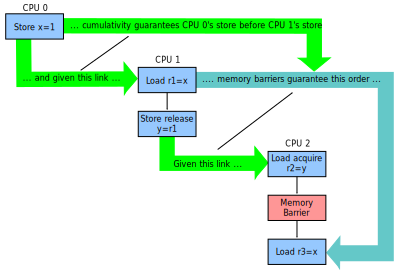
\includegraphics{memorder/memorybarriercum}
\caption{Cumulativity}
\label{fig:memorder:Cumulativity}
\end{figure*}

These ordering constraints are depicted graphically in
Figure~\ref{fig:memorder:Cumulativity}.
Note also that cumulativity is not limited to a single step back in time.
If there was another load from \co{x} or store to \co{x} from any thread
that came before the store on line~13, that prior load or store would also
be ordered before the store on line~32, though only if both \co{r1} and
\co{r2} both end up containing the address of \co{x}.

In short, use of cumulative ordering operations can suppress
non-multicopy-atomic behaviors in some situations.
Cumulativity nevertheless has limits, which are examined in the next section.

\subsubsection{Propagation}
\label{sec:memorder:Propagation}

\begin{listing}[tbp]
{ \scriptsize
\begin{verbbox}[\LstLineNo]
C C-W+RWC+o-r+a-o+o-mb-o

{
int x = 0;
int y = 0;
int z = 0;
}

P0(int *x, int *y)
{
  WRITE_ONCE(*x, 1);
  smp_store_release(y, 1);
}

P1(int *y, int *z)
{
  int r1;
  int r2;

  r1 = smp_load_acquire(y);
  r2 = READ_ONCE(*z);
}

P2(int *z, int *x)
{
  int r3;

  WRITE_ONCE(*z, 1);
  smp_mb();
  r3 = READ_ONCE(*x);
}

exists(1:r1=1 /\ 1:r2=0 /\ 2:r3=0)
\end{verbbox}
}
\centering
\theverbbox
\caption{W+RWC Litmus Test With Release (No Ordering)}
\label{lst:memorder:W+RWC Litmus Test With Release (No Ordering)}
\end{listing}

Listing~\ref{lst:memorder:W+RWC Litmus Test With Release (No Ordering)}
(\path{C-W+RWC+o-r+a-o+o-mb-o.litmus})
shows the limitations of cumulativity and of store-release,
even with a full memory barrier helping out.
The problem is that although the \co{smp_store_release()} on
line~12 has cumulativity, and although that cumulativity does
order \co{P2()}'s load on line~30, the \co{smp_store_release()}'s
ordering cannot propagate through the combination of \co{P1()}'s
load (line~21) and \co{P2()}'s store (line~28).
This means that the \co{exists} clause on line~33 really can trigger.

\QuickQuiz{}
	But it is not necessary to worry about propagation unless
	there are at least three threads in the litmus test, right?
\QuickQuizAnswer{
\begin{listing}[tbp]
{ \scriptsize
\begin{verbbox}[\LstLineNo]
C C-R+o-wmb-o+o-mb-o
{
}

P0(int *x0, int *x1)
{
  WRITE_ONCE(*x0, 1);
  smp_wmb();
  WRITE_ONCE(*x1, 1);
}


P1(int *x0, int *x1)
{
  int r2;

  WRITE_ONCE(*x1, 2);
  smp_mb();
  r2 = READ_ONCE(*x0);
}

exists (1:r2=0 /\ x1=2)
\end{verbbox}
}
\centering
\theverbbox
\caption{R Litmus Test With Write Memory Barrier (No Ordering)}
\label{lst:memorder:R Litmus Test With Write Memory Barrier (No Ordering)}
\end{listing}
	Wrong.

	Listing~\ref{lst:memorder:R Litmus Test With Write Memory Barrier (No Ordering)}
	(\path{C-R+o-wmb-o+o-mb-o.litmus})
	shows a two-thread litmus test that requires propagation due to
	the fact that it only has store-to-store and load-to-store
	relationships between its pair of threads.
	Even though \co{P0()} is fully ordered by the \co{smp_wmb()} and
	\co{P1()} is fully ordered by the \co{smp_mb()}, the
	counter-temporal nature of the relationships means that
	the \co{exists} clause on line~22 really can trigger.
	To prevent this triggering, the \co{smp_wmb()} on line~8
	must become an \co{smp_mb()}, bringing propagation into play
	twice, once for each non-temporal relationship.
} \QuickQuizEnd

\begin{figure}[htbp]
\centering
\resizebox{\columnwidth}{!}{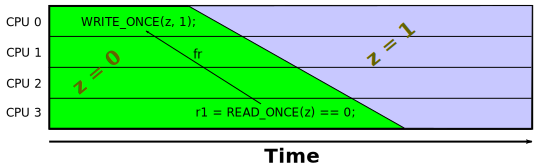
\includegraphics{memorder/fr}}
\caption{Load-to-Store is Counter-Temporal}
\label{fig:memorder:Load-to-Store is Counter-Temporal}
\end{figure}

This situation might seem completely counter-intuitive, but keep
in mind that the speed of light is finite and computers are of
non-zero size.
It therefore takes time for the effect of the \co{P2()}'s store to
\co{z} to propagate to \co{P1()}, which in turn means that it is possible
that \co{P1()}'s read from \co{z} happens much later in time, but
nevertheless still sees the old value of zero.
This situation is depicted in
Figure~\ref{fig:memorder:Load-to-Store is Counter-Temporal}:
Just because a load sees the old value does \emph{not} mean that
this load executed at an earlier time than did the store of the
new value.

Note that
Listing~\ref{lst:memorder:W+RWC Litmus Test With Release (No Ordering)}
also shows the limitations of memory-barrier pairing, given that
there are not two but three processes.
These more complex litmus tests can instead be said to have \emph{cycles},
where memory-barrier pairing is the special case of a two-thread cycle.
The cycle in
Listing~\ref{lst:memorder:W+RWC Litmus Test With Release (No Ordering)}
goes through \co{P0()} (lines~11 and~12), \co{P1()} (lines~20 and~21),
\co{P2()} (lines~28, 29, and~30), and back to \co{P0()} (line~11).
The \co{exists} clause delineates this cycle:
the \co{1:r1=1} indicates that the \co{smp_load_acquire()} on line~20
returned the value stored by the \co{smp_store_release()} on line~12,
the \co{1:r2=0} indicates that the \co{WRITE_ONCE()} on line~28 came
too late to affect the value returned by the \co{READ_ONCE()} on line~21,
and finally the \co{2:r3=0} indicates that the
\co{WRITE_ONCE()} on line~11 came to late to affect the value returned
by the \co{READ_ONCE()} on line~30.
In this case, the fact that the \co{exists} clause can trigger means that
the cycle is said to be \emph{allowed}.
In contrast, in cases where the \co{exists} clause cannot trigger,
the cycle is said to be \emph{prohibited}.

\begin{listing}[tbp]
{ \scriptsize
\begin{verbbox}[\LstLineNo]
C C-W+RWC+o-mb-o+a-o+o-mb-o

{
int x = 0;
int y = 0;
int z = 0;
}

P0(int *x, int *y)
{
  WRITE_ONCE(*x, 1);
  smp_mb();
  WRITE_ONCE(*y, 1);
}

P1(int *y, int *z)
{
  int r1;
  int r2;

  r1 = smp_load_acquire(y);
  r2 = READ_ONCE(*z);
}

P2(int *z, int *x)
{
  int r3;

  WRITE_ONCE(*z, 1);
  smp_mb();
  r3 = READ_ONCE(*x);
}

exists(1:r1=1 /\ 1:r2=0 /\ 2:r3=0)
\end{verbbox}
}
\centering
\theverbbox
\caption{W+WRC Litmus Test With More Barriers}
\label{lst:memorder:W+WRC Litmus Test With More Barriers}
\end{listing}

But what if we need to keep the \co{exists} clause on line~33 of
Listing~\ref{lst:memorder:W+RWC Litmus Test With Release (No Ordering)}?
One solution is to replace \co{P0()}'s \co{smp_store_release()}
with an \co{smp_mb()}, which
Table~\ref{tab:memorder:Linux-Kernel Memory-Ordering Cheat Sheet}
shows to have not only cumulativity, but also propagation.
The result is shown in
Listing~\ref{lst:memorder:W+WRC Litmus Test With More Barriers}
(\path{C-W+RWC+o-mb-o+a-o+o-mb-o.litmus}).

\QuickQuiz{}
	But given that \co{smp_mb()} has the propagation property,
	why doesn't the \co{smp_mb()} on line~29 of
	Listing~\ref{lst:memorder:W+RWC Litmus Test With Release (No Ordering)}
	prevent the \co{exists} clause from triggering?
\QuickQuizAnswer{
	As a rough rule of thumb, the \co{smp_mb()} barrier's
	propagation property is sufficient to maintain ordering
	through only one store-to-load relationship between
	processes.
	Unfortunately,
	Listing~\ref{lst:memorder:W+RWC Litmus Test With Release (No Ordering)}
	has not one but two store-to-load relationships, with the
	first being from the \co{READ_ONCE()} on line~21 to the
	\co{WRITE_ONCE()} on line~28 and the second being from
	the \co{READ_ONCE()} on line~30 to the \co{WRITE_ONCE()}
	on line~11.
	Therefore, preventing the \co{exists} clause from triggering
	should be expected to require not one but two
	instances of \co{smp_mb()}.

	As a special exception to this rule of thumb, a release-acquire
	chain can have one load-to-store relationship between processes
	and still prohibit the cycle.
} \QuickQuizEnd

\begin{figure}[tbp]
\centering
\resizebox{\columnwidth}{!}{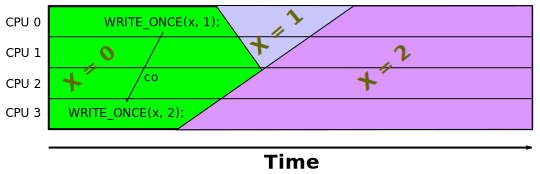
\includegraphics{memorder/co}}
\caption{Store-to-Store is Counter-Temporal}
\label{fig:memorder:Store-to-Store is Counter-Temporal}
\end{figure}

For completeness,
Figure~\ref{fig:memorder:Store-to-Store is Counter-Temporal}
shows that the ``winning'' store among a group of stores to the
same variable is not necessarily the store that started last.
This should not come as a surprise to anyone who carefully examined
Figure~\ref{fig:memorder:A Variable With More Simultaneous Values}.

But sometimes time is on our side, as shown in the next section.

\subsubsection{Happens-Before}
\label{sec:memorder:Happens-Before}

\begin{figure}[tbp]
\centering
\resizebox{\columnwidth}{!}{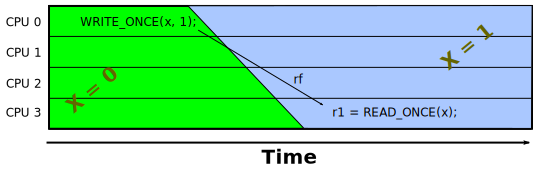
\includegraphics{memorder/rf}}
\caption{Store-to-Load is Temporal}
\label{fig:memorder:Store-to-Load is Temporal}
\end{figure}

As shown in
Figure~\ref{fig:memorder:Store-to-Load is Temporal},
on non-speculative platforms, if a load returns the value from a
particular store, then, courtesy of the finite speed of light and
the non-zero size of modern computing systems, the store absolutely
has to have executed at an earlier time than did the load.
This means that carefully constructed programs can rely on the
passage of time itself as an memory-ordering operation.

\begin{listing}[tbp]
{ \scriptsize
\begin{verbbox}[\LstLineNo]
C C-LB+a-o+o-data-o+o-data-o
{
}

P0(int *x0, int *x1)
{
  int r2;

  r2 = smp_load_acquire(x0);
  WRITE_ONCE(*x1, 2);
}


P1(int *x1, int *x2)
{
  int r2;

  r2 = READ_ONCE(*x1);
  WRITE_ONCE(*x2, r2);
}

P2(int *x2, int *x0)
{
  int r2;

  r2 = READ_ONCE(*x2);
  WRITE_ONCE(*x0, r2);
}

exists (0:r2=2 /\ 1:r2=2 /\ 2:r2=2)
\end{verbbox}
}
\centering
\theverbbox
\caption{LB Litmus Test With One Acquire}
\label{lst:memorder:LB Litmus Test With One Acquire}
\end{listing}

Of course, just the passage of time by itself is not enough, as
was seen in
Listing~\ref{lst:memorder:Load-Buffering Litmus Test (No Ordering)},
which has nothing but store-to-load relationships and still can
trigger its \co{exists} clause.
However, as long as each thread provides even the weakest possible
ordering, \co{exists} clause would not be able to trigger.
For example,
Listing~\ref{lst:memorder:LB Litmus Test With One Acquire}
(\path{C-LB+a-o+o-data-o+o-data-o.litmus})
shows \co{P0()} ordered with an \co{smp_load_acquire()} and
both \co{P1()} and \co{P2()} ordered with data dependencies.
These orderings, which are close to the top of
Table~\ref{tab:memorder:Linux-Kernel Memory-Ordering Cheat Sheet},
suffice to prevent the \co{exists} clause from triggering.

\QuickQuiz{}
	Can you construct a litmus test similar to that in
	Listing~\ref{lst:memorder:LB Litmus Test With One Acquire}
	that uses \emph{only} dependencies?
\QuickQuizAnswer{
	Listing~\ref{lst:memorder:LB Litmus Test With No Acquires}
	shows a somewhat nonsensical but very real example.
	Creating a more useful (but still real) litmus test is left
	as an exercise for the reader.
\begin{listing}[tbp]
{ \scriptsize
\begin{verbbox}[\LstLineNo]
C C-LB+o-data-o+o-data-o+o-data-o
{
int x0=0;
int x1=1;
int x2=2;
}

P0(int *x0, int *x1)
{
  int r2;

  r2 = READ_ONCE(*x0);
  WRITE_ONCE(*x1, r2);
}


P1(int *x1, int *x2)
{
  int r2;

  r2 = READ_ONCE(*x1);
  WRITE_ONCE(*x2, r2);
}

P2(int *x2, int *x0)
{
  int r2;

  r2 = READ_ONCE(*x2);
  WRITE_ONCE(*x0, r2);
}

exists (0:r2=2 /\ 1:r2=0 /\ 2:r2=1)
\end{verbbox}
}
\centering
\theverbbox
\caption{LB Litmus Test With No Acquires}
\label{lst:memorder:LB Litmus Test With No Acquires}
\end{listing}
} \QuickQuizEnd

An important, to say nothing of more useful, use of time for ordering
memory accesses is covered in the next section.

\subsubsection{Release-Acquire Chains}
\label{sec:memorder:Release-Acquire Chains}

\begin{listing}[tbp]
{ \scriptsize
\begin{verbbox}[\LstLineNo]
C C-LB+a-r+a-r+a-r+a-r
{
}

P0(int *x0, int *x1)
{
  int r2;

  r2 = smp_load_acquire(x0);
  smp_store_release(x1, 2);
}


P1(int *x1, int *x2)
{
  int r2;

  r2 = smp_load_acquire(x1);
  smp_store_release(x2, 2);
}

P2(int *x2, int *x3)
{
  int r2;

  r2 = smp_load_acquire(x2);
  smp_store_release(x3, 2);
}

P3(int *x3, int *x0)
{
  int r2;

  r2 = smp_load_acquire(x3);
  smp_store_release(x0, 2);
}

exists (0:r2=2 /\ 1:r2=2 /\ 2:r2=2 /\ 3:r2=2)
\end{verbbox}
}
\centering
\theverbbox
\caption{Long LB Release-Acquire Chain}
\label{lst:memorder:Long LB Release-Acquire Chain}
\end{listing}

A minimal release-acquire chain was shown in
Listing~\ref{lst:memorder:Enforcing Ordering of Load-Buffering Litmus Test}
(\path{C-LB+a-r+a-r+a-r+a-r.litmus}),
but these chains can be much longer, as shown in
Listing~\ref{lst:memorder:Long LB Release-Acquire Chain}.
The longer the release-acquire chain, the more benefit is gained
from the passage of time, so that no matter how many threads are
involved, the corresponding \co{exists} clause cannot trigger..
Give or take the increased computational demands of the larger number
of threads, of course!

\begin{listing}[tbp]
{ \scriptsize
\begin{verbbox}[\LstLineNo]
C C-ISA2+o-r+a-r+a-r+a-o
{
}

P0(int *x0, int *x1)
{
  WRITE_ONCE(*x0, 2);
  smp_store_release(x1, 2);
}


P1(int *x1, int *x2)
{
  int r2;

  r2 = smp_load_acquire(x1);
  smp_store_release(x2, 2);
}

P2(int *x2, int *x3)
{
  int r2;

  r2 = smp_load_acquire(x2);
  smp_store_release(x3, 2);
}

P3(int *x3, int *x0)
{
  int r1;
  int r2;

  r1 = smp_load_acquire(x3);
  r2 = READ_ONCE(*x0);
}

exists (1:r2=2 /\ 2:r2=2 /\ 3:r1=2 /\ 3:r2=0)
\end{verbbox}
}
\centering
\theverbbox
\caption{Long ISA2 Release-Acquire Chain}
\label{lst:memorder:Long ISA2 Release-Acquire Chain}
\end{listing}

Although release-acquire chains are inherently store-to-load creatures,
it turns out that they can tolerate one load-to-store step, despite
such steps being counter-temporal, as shown in
Figure~\ref{fig:memorder:Load-to-Store is Counter-Temporal}.
For example,
Listing~\ref{lst:memorder:Long ISA2 Release-Acquire Chain}
(\path{C-ISA2+o-r+a-r+a-r+a-o.litmus})
shows a three-step release-acquire chain, but where \co{P3()}'s
final access is a \co{READ_ONCE()} from \co{x0}, which is
accessed via \co{WRITE_ONCE()} by \co{P0()}, forming a non-temporal
load-to-store relationship between these two processes.
However, because \co{P0()}'s \co{smp_store_release()} (line~12)
is cumulative, if \co{P3()}'s \co{READ_ONCE()} returns zero,
this cumulativity will force the \co{READ_ONCE()} to be ordered
before \co{P0()}'s \co{smp_store_release()}.
However, the release-acquire chain (lines~12, 20, 21, 28, 29, and~37)
forces \co{P3()}'s \co{READ_ONCE()} to be ordered after \co{P0()}'s
\co{smp_store_release()}.
Because \co{P3()}'s \co{READ_ONCE()} cannot be both before and after
\co{P0()}'s \co{smp_store_release()}, either or both of two things must
be true:

\begin{enumerate}
\item	\co{P3()}'s \co{READ_ONCE()} came after \co{P0()}'s
	\co{WRITE_ONCE()}, so that the \co{READ_ONCE()} returned
	the value two, so that the \co{exists} clause's \co{3:r2=0}
	is false.
\item	The release-acquire chain did not form, that is, one or more
	of the \co{exists} clause's \co{1:r2=2}, \co{2:r2=2}, or \co{3:r1=2}
	is false.
\end{enumerate}

Either way, the \co{exists} clause cannot trigger, despite this litmus
test containing a notorious load-to-store relationship between
\co{P3()} and \co{P0()}.
But never forget that release-acquire chains can tolerate only one
load-to-store relationship, as was seen in
Listing~\ref{lst:memorder:W+RWC Litmus Test With Release (No Ordering)}.

\begin{listing}[tbp]
{ \scriptsize
\begin{verbbox}[\LstLineNo]
C C-Z6.2+o-r+a-r+a-r+a-o
{
}

P0(int *x0, int *x1)
{
  WRITE_ONCE(*x0, 2);
  smp_store_release(x1, 2);
}


P1(int *x1, int *x2)
{
  int r2;

  r2 = smp_load_acquire(x1);
  smp_store_release(x2, 2);
}

P2(int *x2, int *x3)
{
  int r2;

  r2 = smp_load_acquire(x2);
  smp_store_release(x3, 2);
}

P3(int *x3, int *x0)
{
  int r2;

  r2 = smp_load_acquire(x3);
  WRITE_ONCE(*x0, 3);
}

exists (1:r2=2 /\ 2:r2=2 /\ 3:r2=2 /\ x0=2)
\end{verbbox}
}
\centering
\theverbbox
\caption{Long Z6.2 Release-Acquire Chain}
\label{lst:memorder:Long Z6.2 Release-Acquire Chain}
\end{listing}

Release-acquire chains can also tolerate a single store-to-store step,
as shown in
Listing~\ref{lst:memorder:Long Z6.2 Release-Acquire Chain}
(\path{C-Z6.2+o-r+a-r+a-r+a-o.litmus}).
As with the previous example, \co{smp_store_release()}'s cumulativity
combined with the temporal nature of the release-acquire chain
prevents the \co{exists} clause on line~36 from triggering.
But beware: Adding a second store-to-store step would allow the correspondingly
updated \co{exists} clause to trigger.

% @@@ QQ on having a release-acquire chain with one load-to-store and
% @@@ one store-to-store relationship.

In short, properly constructed release-acquire chains form a peaceful
island of intuitive bliss surrounded by a strongly counter-intuitive
sea of more complex memory-ordering constraints.

% Exercises?
% Hardware details from Appendix?

\section{Compile-Time Consternation}
\label{sec:memorder:Compile-Time Consternation}

\subsection{Memory-Reference Restrictions}
\label{sec:memorder:Memory-Reference Restrictions}

% @@@ Section on READ_ONCE() and WRITE_ONCE()
% @@@ Convert some examples in "restrictions" sections to litmus tests

\subsection{Address- and Data-Dependency Restrictions}
\label{sec:memorder:Address- and Data-Dependency Restrictions}

Compilers do not understand either address or data dependencies,
although there are efforts underway to teach them, or at the very
least, standardize the process of teaching
them~\cite{PaulEMcKennneyConsumeP0190R0,PaulEMcKenney2017markconsumeP0462R1}.
In the meantime, it is necessary to be very careful in order to avoid
giving your compiler the opportunity to break your dependencies.

\subsubsection{Give your dependency chain a good start}
The load that heads your dependency chain must use proper
ordering, for example, \co{lockless_dereference()},
\co{rcu_dereference()}, or
a \co{READ_ONCE()} followed by \co{smp_read_barrier_depends()}.
Failure to follow this rule can have serious side effects:

\begin{enumerate}
\item	On DEC Alpha, a dependent load might not be ordered with
	the load heading the dependency chain, as described in
	Section~\ref{sec:app:whymb:Alpha}.
\item	If the load heading the dependency chain is a
	C11 non-volatile \co{memory_order_relaxed} load,
	the compiler could omit the load, for example, by using a value
	that it loaded in the past.
\item	If the load heading the dependency chain is a plain load,
	the compiler can omit the load, again by using a value
	that it loaded in the past.
	Worse yet, it could load twice instead of once, so that
	different parts of your code use different values---and
	real compilers do this, especially when under register
	pressure.
\item	The value loaded by the head of the dependency chain must
	be a pointer.
	In theory, yes, you could load an integer, perhaps to use
	it as an array index.
	In practice, the compiler knows too much about integers,
	and thus has way too many opportunities to break your
	dependency chain.
\end{enumerate}

\subsubsection{Avoid arithmetic dependency breakage}
Although it is just fine to do some arithmetic operations on a pointer in
your dependency chain, you need to be careful to avoid giving the
compiler too much information.
After all, if the compiler learns enough to determine the exact value
of the pointer, it can and sometimes will use that exact value instead
of the pointer itself.
As soon as the compiler does that, the dependency is broken and all
ordering is lost.

\begin{figure}[tbp]
{ \scriptsize
\begin{verbbox}
 1 int reserve_int;
 2 int *gp;
 3 int *p;
 4
 5 p = rcu_dereference(gp);
 6 if (p == &reserve_int)
 7   handle_reserve(p);
 8 do_something_with(*p); /* buggy! */
\end{verbbox}
}
\centering
\theverbbox
\caption{Breakable Dependencies With Comparisons}
\label{fig:memorder:Breakable Dependencies With Comparisons}
\end{figure}

\begin{figure}[tbp]
{ \scriptsize
\begin{verbbox}
 1 int reserve_int;
 2 int *gp;
 3 int *p;
 4
 5 p = rcu_dereference(gp);
 6 if (p == &reserve_int) {
 7   handle_reserve(&reserve_int);
 8   do_something_with(reserve_int); /* buggy! */
 9 } else {
10   do_something_with(*p); /* OK! */
11 }
\end{verbbox}
}
\centering
\theverbbox
\caption{Broken Dependencies With Comparisons}
\label{fig:memorder:Broken Dependencies With Comparisons}
\end{figure}

\begin{enumerate}
\item	Although it is permissible to compute offsets from a
	pointer, these offsets must not result in total cancellation.
	For example, given a \co{char} pointer \co{cp},
	\co{cp-(uintptr_t)cp)} will cancel and can allow the compiler
	to break your dependency chain.
	On the other hand, canceling offset values with each other
	is perfectly safe and legal.
	For example, if \co{a} and \co{b} are equal, \co{cp+a-b}
	is an identity function, including preserving the dependency.
\item	Comparisons can break dependencies.
	Figure~\ref{fig:memorder:Breakable Dependencies With Comparisons}
	shows how this can happen.
	Here global pointer \co{gp} points to a dynamically allocated
	integer, but if memory is low, it might instead point to
	the \co{reserve_int} variable.
	This \co{reserve_int} case might need special handling, as
	shown on lines~6 and~7 of the figure.
	But the compiler could reasonably transform this code into
	the form shown in
	Figure~\ref{fig:memorder:Broken Dependencies With Comparisons},
	especially on systems where instructions with absolute
	addresses run faster than instructions using addresses
	supplied in registers.
	However, there is clearly no ordering between the pointer
	load on line~5 and the dereference on line~8.
	Please note that this is simply an example: There are a great
	many other ways to break dependency chains with comparisons.
\end{enumerate}

\QuickQuiz{}
	Why can't you simply dereference the pointer before comparing it
	to \co{&reserve_int} on line~6 of
	Figure~\ref{fig:memorder:Breakable Dependencies With Comparisons}?
\QuickQuizAnswer{
	For first, it might be necessary to invoke
	\co{handle_reserve()} before \co{do_something_with()}.

	But more relevant to memory ordering, the compiler is often within
	its rights to hoist the comparison ahead of the dereferences,
	which would allow the compiler to use \co{&reserve_int} instead
	of the varaiable \co{p} that the hardware has tagged with
	a dependency.
} \QuickQuizEnd

\QuickQuiz{}
	But it should be safe to compare two pointer variables,
	right?  After all, the compiler doesn't know the value
	of either, so how can it possibly learn anything from the
	comparison?
\QuickQuizAnswer{

\begin{figure}[tbp]
{ \scriptsize
\begin{verbbox}
 1 int *gp1;
 2 int *gp2;
 3 int *p;
 4 int *q;
 5
 6 p = rcu_dereference(gp1);
 7 q = READ_ONCE(gp2);
 8 if (p == q)
 9   handle_equality(p);
10 do_something_with(*p);
\end{verbbox}
}
\centering
\theverbbox
\caption{Breakable Dependencies With Non-Constant Comparisons}
\label{fig:memorder:Breakable Dependencies With Non-Constant Comparisons}
\end{figure}

\begin{figure}[tbp]
{ \scriptsize
\begin{verbbox}
 1 int *gp1;
 2 int *gp2;
 3 int *p;
 4 int *q;
 5
 6 p = rcu_dereference(gp1);
 7 q = READ_ONCE(gp2);
 8 if (p == q) {
 9   handle_equality(q);
10   do_something_with(*q);
11 } else {
12   do_something_with(*p);
13 }
\end{verbbox}
}
\centering
\theverbbox
\caption{Broken Dependencies With Non-Constant Comparisons}
\label{fig:memorder:Broken Dependencies With Non-Constant Comparisons}
\end{figure}

	Unfortunately, the compiler really can learn enough to
	break your dependency chain, for example, as shown in
	Figure~\ref{fig:memorder:Breakable Dependencies With Non-Constant Comparisons}.
	The compiler is within its rights to transform this code
	into that shown in
	Figure~\ref{fig:memorder:Broken Dependencies With Non-Constant Comparisons},
	and might well make this transformation due to register pressure
	if \co{handle_equality()} was inlined and needed a lot of registers.
	Line~10 of this transformed code uses \co{q}, which although
	equal to \co{p}, is not necessarily tagged by the hardware as
	carrying a dependency.
	Therefore, this transformed code does not necessarily guarantee
	that line~10 is ordered after line~6.\footnote{
		Kudos to Linus Torvalds for providing this example.}
} \QuickQuizEnd

% @@@ Quick quiz showing other ways to break dependencies by comparison

\subsubsection{Safe comparison of dependent pointers}
It turns out that there are several safe ways to compare dependent
pointers:

\begin{enumerate}
\item	Comparisons against the \co{NULL} pointer.
	In this case, all the compiler can learn is that the pointer
	is \co{NULL}, in which case you are not allowed to
	dereference it in any case.
\item	The dependent pointer is never dereferenced, whether before or
	after the comparison.
\item	The dependent pointer is compared to a pointer that references
	objects that were last modified a very long time ago, where
	the safest value of ``a very long time ago'' is at compile time.
\end{enumerate}

@@@ convert to \co{uintptr_t} to set/clear bits and convert back.

% @@@ More here

\subsection{Control-Dependency Restrictions}
\label{sec:memorder:Control-Dependency Restrictions}

Control dependencies are especially tricky because current compilers
do not understand them and can easily break them.
The rules and examples in this section are intended to help you
prevent your compiler's ignorance from breaking your code.

A load-load control dependency requires a full read memory barrier,
not simply a data dependency barrier.
Consider the following bit of code:

\vspace{5pt}
\begin{minipage}[t]{\columnwidth}
\scriptsize
\begin{verbatim}
  1 q = READ_ONCE(x);
  2 if (q) {
  3   <data dependency barrier>
  4   q = READ_ONCE(y);
  5 }
\end{verbatim}
\end{minipage}
\vspace{5pt}

This will not have the desired effect because there is no actual data
dependency, but rather a control dependency that the CPU may short-circuit
by attempting to predict the outcome in advance, so that other CPUs see
the load from~\co{y} as having happened before the load from~\co{x}.
In such a case what's actually required is:

\vspace{5pt}
\begin{minipage}[t]{\columnwidth}
\scriptsize
\begin{verbatim}
  1 q = READ_ONCE(x);
  2 if (q) {
  3   <read barrier>
  4   q = READ_ONCE(y);
  5 }
\end{verbatim}
\end{minipage}
\vspace{5pt}

However, stores are not speculated.
This means that ordering \emph{is} provided for load-store control
dependencies, as in the following example:

\vspace{5pt}
\begin{minipage}[t]{\columnwidth}
\scriptsize
\begin{verbatim}
  1 q = READ_ONCE(x);
  2 if (q)
  3   WRITE_ONCE(y, 1);
\end{verbatim}
\end{minipage}
\vspace{5pt}

Control dependencies pair normally with other types of barriers.
That said, please note that neither \co{READ_ONCE()} nor \co{WRITE_ONCE()}
are optional!
Without the \co{READ_ONCE()}, the compiler might combine the load
from~\co{x} with other loads from~\co{x}.
Without the \co{WRITE_ONCE()}, the compiler might combine the store
to~\co{y} with other stores to~\co{y}.
Either can result in highly counterintuitive effects on ordering.

Worse yet, if the compiler is able to prove (say) that the value of
variable~\co{x} is always non-zero, it would be well within its rights
to optimize the original example by eliminating the ``\co{if}'' statement
as follows:

\vspace{5pt}
\begin{minipage}[t]{\columnwidth}
\scriptsize
\begin{verbatim}
  1 q = READ_ONCE(x);
  2 WRITE_ONCE(y, 1); /* BUG: CPU can reorder!!! */
\end{verbatim}
\end{minipage}
\vspace{5pt}

It is tempting to try to enforce ordering on identical stores on both
branches of the ``\co{if}'' statement as follows:

\vspace{5pt}
\begin{minipage}[t]{\columnwidth}
\scriptsize
\begin{verbatim}
 1 q = READ_ONCE(x);
 2 if (q) {
 3   barrier();
 4   WRITE_ONCE(y, 1);
 5   do_something();
 6 } else {
 7   barrier();
 8   WRITE_ONCE(y, 1);
 9   do_something_else();
10 }
\end{verbatim}
\end{minipage}
\vspace{5pt}

Unfortunately, current compilers will transform this as follows at high
optimization levels:

\vspace{5pt}
\begin{minipage}[t]{\columnwidth}
\scriptsize
\begin{verbatim}
 1 q = READ_ONCE(x);
 2 barrier();
 3 WRITE_ONCE(y, 1);  /* BUG: No ordering!!! */
 4 if (q) {
 5   do_something();
 6 } else {
 7   do_something_else();
 8 }
\end{verbatim}
\end{minipage}
\vspace{5pt}

Now there is no conditional between the load from~\co{x} and the store
to~\co{y}, which means that the CPU is within its rights to reorder them:
The conditional is absolutely required, and must be present in the
assembly code even after all compiler optimizations have been applied.
Therefore, if you need ordering in this example, you need explicit
memory barriers, for example, a release store:

\vspace{5pt}
\begin{minipage}[t]{\columnwidth}
\scriptsize
\begin{verbatim}
 1 q = READ_ONCE(x);
 2 if (q) {
 3   smp_store_release(&y, 1);
 4   do_something();
 5 } else {
 6   smp_store_release(&y, 1);
 7   do_something_else();
 8 }
\end{verbatim}
\end{minipage}
\vspace{5pt}

The initial \co{READ_ONCE()} is still required to prevent the compiler from
proving the value of~\co{x}.

In addition, you need to be careful what you do with the local variable~%
\co{q},
otherwise the compiler might be able to guess the value and again remove
the needed conditional.
For example:

\vspace{5pt}
\begin{minipage}[t]{\columnwidth}
\scriptsize
\begin{verbatim}
 1 q = READ_ONCE(x);
 2 if (q % MAX) {
 3   WRITE_ONCE(y, 1);
 4   do_something();
 5 } else {
 6   WRITE_ONCE(y, 2);
 7   do_something_else();
 8 }
\end{verbatim}
\end{minipage}
\vspace{5pt}

If \co{MAX} is defined to be~1, then the compiler knows that \co{(q\%MAX)} is
equal to zero, in which case the compiler is within its rights to
transform the above code into the following:

\vspace{5pt}
\begin{minipage}[t]{\columnwidth}
\scriptsize
\begin{verbatim}
 1 q = READ_ONCE(x);
 2 WRITE_ONCE(y, 2);
 3 do_something_else();
\end{verbatim}
\end{minipage}
\vspace{5pt}

Given this transformation, the CPU is not required to respect the ordering
between the load from variable~\co{x} and the store to variable~\co{y}.
It is tempting to add a \co{barrier()} to constrain the compiler,
but this does not help.
The conditional is gone, and the barrier won't bring it back.
Therefore, if you are relying on this ordering, you should make sure
that \co{MAX} is greater than one, perhaps as follows:

\vspace{5pt}
\begin{minipage}[t]{\columnwidth}
\scriptsize
\begin{verbatim}
 1 q = READ_ONCE(x);
 2 BUILD_BUG_ON(MAX <= 1);
 3 if (q % MAX) {
 4   WRITE_ONCE(y, 1);
 5   do_something();
 6 } else {
 7   WRITE_ONCE(y, 2);
 8   do_something_else();
 9 }
\end{verbatim}
\end{minipage}
\vspace{5pt}

Please note once again that the stores to~\co{y} differ.
If they were identical, as noted earlier, the compiler could pull this
store outside of the ``\co{if}'' statement.

You must also avoid excessive reliance on boolean short-circuit evaluation.
Consider this example:

\vspace{5pt}
\begin{minipage}[t]{\columnwidth}
\scriptsize
\begin{verbatim}
 1 q = READ_ONCE(x);
 2 if (q || 1 > 0)
 3   WRITE_ONCE(y, 1);
\end{verbatim}
\end{minipage}
\vspace{5pt}

Because the first condition cannot fault and the second condition is
always true, the compiler can transform this example as following,
defeating control dependency:

\vspace{5pt}
\begin{minipage}[t]{\columnwidth}
\scriptsize
\begin{verbatim}
 1 q = READ_ONCE(x);
 2 WRITE_ONCE(y, 1);
\end{verbatim}
\end{minipage}
\vspace{5pt}

This example underscores the need to ensure that the compiler cannot
out-guess your code.
More generally, although \co{READ_ONCE()} does force
the compiler to actually emit code for a given load, it does not force
the compiler to use the results.

In addition, control dependencies apply only to the then-clause and
else-clause of the if-statement in question.
In particular, it does
not necessarily apply to code following the if-statement:

\vspace{5pt}
\begin{minipage}[t]{\columnwidth}
\scriptsize
\begin{verbatim}
 1 q = READ_ONCE(x);
 2 if (q) {
 3   WRITE_ONCE(y, 1);
 4 } else {
 5   WRITE_ONCE(y, 2);
 6 }
 7 WRITE_ONCE(z, 1);  /* BUG: No ordering. */
\end{verbatim}
\end{minipage}
\vspace{5pt}

It is tempting to argue that there in fact is ordering because the
compiler cannot reorder volatile accesses and also cannot reorder
the writes to~\co{y} with the condition.
Unfortunately for this line
of reasoning, the compiler might compile the two writes to~\co{y} as
conditional-move instructions, as in this fanciful pseudo-assembly
language:

\vspace{5pt}
\begin{minipage}[t]{\columnwidth}
\scriptsize
\begin{verbatim}
 1 ld r1,x
 2 cmp r1,$0
 3 cmov,ne r4,$1
 4 cmov,eq r4,$2
 5 st r4,y
 6 st $1,z
\end{verbatim}
\end{minipage}
\vspace{5pt}

A weakly ordered CPU would have no dependency of any sort between the load
from~\co{x} and the store to~\co{z}.
The control dependencies would extend
only to the pair of cmov instructions and the store depending on them.
In short, control dependencies apply only to the stores in the ``\co{then}''
and ``\co{else}'' of the ``\co{if}'' in question (including functions
invoked by those two clauses), not to code following that ``\co{if}''.

Finally, control dependencies do \emph{not} provide cumulativity.\footnote{
	Refer to Section~\ref{sec:memorder:Cumulativity} for
	the meaning of transitivity.}
This is demonstrated by two related examples, with the initial values
of~\co{x} and~\co{y} both being zero:

\vspace{5pt}
\begin{minipage}[t]{\columnwidth}
\tt
\scriptsize
\begin{tabular}{l|p{1.5in}}
	\nf{CPU 0} &	\nf{CPU 1} \\
	\hline
	\tco{r1 = READ_ONCE(x);} &
		\tco{r2 = READ_ONCE(y);} \\
	if (r1 > 0) &
		if (r2 > 0) \\
	~~~\tco{WRITE_ONCE(y, 1);} &
		~~~\tco{WRITE_ONCE(x, 1);} \\
	\multicolumn{2}{l}{~} \\
	\multicolumn{2}{l}{\tco{assert(!(r1 == 1 && r2 == 1));}} \\
\end{tabular}
\end{minipage}
\vspace{5pt}

The above two-CPU example will never trigger the \co{assert()}.
However, if control dependencies guaranteed transitivity (which they do
not), then adding the following CPU would guarantee a related assertion:

\vspace{5pt}
\begin{minipage}[t]{\columnwidth}
\tt
\scriptsize
\begin{tabular}{l}
	\nf{CPU 2} \\
	\hline
	\tco{WRITE_ONCE(x, 2);} \\
	\multicolumn{1}{l}{~} \\
	\multicolumn{1}{l}{\tco{assert(!(r1 == 2 && r2 == 1 && x == 2));}} \\
\end{tabular}
\end{minipage}
\vspace{5pt}

But because control dependencies do \emph{not} provide transitivity, the above
assertion can fail after the combined three-CPU example completes.
If you need the three-CPU example to provide ordering, you will need
\co{smp_mb()} between the loads and stores in the CPU~0 and CPU~1 code
fragments, that is, just before or just after the ``\co{if}'' statements.
Furthermore, the original two-CPU example is very fragile and should be avoided.

The two-CPU example is known as LB (load buffering) and the three-CPU
example as WWC~\cite{Maranget2012TutorialARMPower}.

The following list of rules summarizes the lessons of this section:

\begin{enumerate}
\item	Compilers do not understand control dependencies, so it is
	your job to make sure that the compiler cannot break your code.

\item	Control dependencies can order prior loads against later stores.
	However, they do \emph{not} guarantee any other sort of ordering:
	Not prior loads against later loads, nor prior stores against
	later anything.
	If you need these other forms of ordering, use \co{smp_rmb()},
	\co{smp_wmb()}, or, in the case of prior stores and later loads,
	\co{smp_mb()}.

\item	If both legs of the ``\co{if}'' statement begin with identical stores
	to the same variable, then those stores must be ordered,
	either by preceding both of them with \co{smp_mb()} or by using
	\co{smp_store_release()} to carry out the stores.
	Please note that it is \emph{not} sufficient to use \co{barrier()}
	at beginning of each leg of the ``\co{if}'' statement because, as shown
	by the example above, optimizing compilers can destroy the control
	dependency while respecting the letter of the \co{barrier()} law.

\item	Control dependencies require at least one run-time conditional
	between the prior load and the subsequent store, and this
	conditional must involve the prior load.
	If the compiler is able to optimize the conditional away, it
	will have also optimized away the ordering.
	Careful use of \co{READ_ONCE()} and \co{WRITE_ONCE()} can help
	to preserve the needed conditional.

\item	Control dependencies require that the compiler avoid reordering
	the dependency into nonexistence.
	Careful use of \co{READ_ONCE()}, \co{atomic_read()}, or
	\co{atomic64_read()} can help to preserve your control
	dependency.

\item	Control dependencies apply only to the ``\co{then}'' and
	``\co{else}'' of the ``\co{if}'' containing the control
	dependency, including any functions that these two clauses call.
	Control dependencies do \emph{not} apply to code following the
	``\co{if}'' containing the control dependency.

\item	Control dependencies pair normally with other types of barriers.

\item	Control dependencies do \emph{not} provide transitivity.
	If you need transitivity, use \co{smp_mb()}.
\end{enumerate}

In short, many popular languages were designed primarily with
single-threaded use in mind.
Successfully using these languages to construct multi-threaded software
requires that you pay special attention to your memory references and
dependencies.

\section{Where is Memory Ordering Needed?}
\label{sec:memorder:Where is Memory Ordering Needed?}

This section revisits
Table~\ref{tab:memorder:Linux-Kernel Memory-Ordering Cheat Sheet}
in light of the intervening discussion.

Memory-ordering operations are only required where there's a possibility
of interaction involving at least two variables between at least two
threads.
As always, if a single-threaded program will provide sufficient
performance, why bother with parallelism?\footnote{
	Hobbyists and researchers should of course feel free to ignore
	this and other cautions.}
After all, avoiding parallelism also avoids the added cost of
memory-ordering operations.

If all your thread-to-thread communication uses store-to-load relationships
(that is, one thread's load returning the value that some other thread
stored), minimal ordering suffices.
Minimal ordering includes dependencies, acquires, and any stronger
ordering operation.

If all but one of your thread-to-thread communications use store-to-load
relationships, release-acquire links for all the store-to-load
relationships suffice.
You can replace acquire with a dependency in environments permitting
this, keeping in mind that the C11 standard memory model does \emph{not}
permit this.
Note also that a dependency leading to a load must be headed by
a \co{lockless_dereference()} or an \co{rcu_dereference()}:
\co{READ_ONCE()} is not sufficient.
Never forget to carefully review
Sections~\ref{sec:memorder:Address- and Data-Dependency Restrictions}
and~\ref{sec:memorder:Control-Dependency Restrictions}.
A dependency broken by your compiler is no help at all!

If two or more of your thread-to-thread communications use something other
than store-to-load relationships, you will need at least one strong barrier
for each load-to-store and for each store-to-store relationship.
Strong barriers include \co{smp_mb()}, successful full-strength non-\co{void}
atomic RMW operations, and other atomic RMW operations in conjunction with
either \co{smp_mb__before_atomic()} or \co{smp_mb__after_atomic()}.
With strength comes expense, though the overhead of strong barriers
usually hurts performance more than it hurts scalability.

Note that these are the \emph{minimum} guarantees.
Different architectures may give
more substantial guarantees,
\IfInBook{as discussed in Appendix~\ref{chp:app:whymb:Why Memory Barriers?},}{}
but they may \emph{not}
be relied upon outside of code specifically designed to run only on
the corresponding architecture.

One final word of advice: Again, use of raw memory-barrier primitives is
a last resort.
It is almost always better to use existing primitives, such as locking
or RCU, that take care of memory ordering for you.
